

\section{Design considerations}

In order for the JIT mechanism to work and fulfill the given requirements, we have come up with a set of necessary components that facilitate the workflow. As depicted in \autoref{fig:jit_module} under \texttt{models}, we have the essential components responsible for representing and managing the models as Python objects before making them available to the NestKernel. The \texttt{jit\_model} stores information about the chosen NESTML model by storing its parameters and state and making it possible for the user to query and change attributes after creating instances. Secondly, we have the \texttt{model\_query}, which is important for searching the model either in the \texttt{.nestml} files or in the created libraries. Depending on the format, the \texttt{model\_query} returns an instance of the \texttt{model\_handle}, which is responsible for making the model available to the NestKernel. The \texttt{model\_handle} knows if the model is coming from a \texttt{.nestml} file, in which case it can initiate the code generation process and install the model, or, if the model is coming from an already existing library, it will just install the model. The \texttt{model\_manager} is responsible for storing all created objects in the JIT module, and it is the only point of communication with the PyNEST module. The \texttt{model\_manager} also manages the mapping between \emph{IDs} of the created models on the Python side and the real models coming from the NestKernel with the help of the \texttt{model\_indexer}. Finally, we have the \texttt{node\_collection\_proxy} that mimics the behavior of the \texttt{NodeCollection} object in PyNEST and provides things like \emph{getters}, \emph{setters}, and code for \emph{indexing} and \emph{slicing}. The need for such a class will be explained later on in this chapter.

\begin{figure}[ht!]
\centering
\resizebox{\textwidth}{!}{
    \begin{tikzpicture}[
      level 1/.style={sibling distance=50mm},
      edge from parent/.style={->,draw},
      >=latex]

    % root of the the initial tree, level 1
    \node[root] {JIT}
    % The first level, as children of the initial tree
      child {node[level 2] (c1) {interfaces}}
      child {node[level 2] (c2) {models}}
      child {node[level 2] (c3) {utils}}
      child {node[level 2] (c4) {wrapper}}
      child {node[level 2] (c5) {nest\_manager.py}}
      child {node[level 2] (c6) {\_\_init\_\_.py}};

    % The second level, relatively positioned nodes
    \begin{scope}[every node/.style={level 3}]
    \node [below of = c1, xshift=25pt] (c11) {jit\_interface.py};

    \node [below of = c2, xshift=25pt] (c21) {jit\_model.py};
    \node [below of = c21] (c22) {model\_query.py};
    \node [below of = c22] (c23) {model\_indexer.py};
    \node [below of = c23] (c24) {model\_manager.py};
    \node [below of = c24] (c25) {model\_handle.py};
    \node [below of = c25] (c26) {node\_collection\_proxy.py};


    \node [below of = c3, xshift=25pt, fill=red!20] (c31) {templates};
    \node [below of = c31] (c32) {report.py};
    \node [below of = c32] (c33) {jit\_model\_parser.py};
    \node [below of = c33] (c34) {nest\_config.py};
    \node [below of = c34] (c35) {symbols.py};
    \node [below of = c35] (c36) {thread\_manager.py};
    \node [below of = c36] (c37) {utils.py};


    \node [below of = c4, xshift=25pt] (c41) {wrapper.py};
    \node [below of = c41] (c42) {wrappers.py};
    \node [below of = c42] (c43) {module\_wrapper.py};


    \end{scope}

    % lines from each level 1 node to every one of its "children"
    \foreach \value in {1}
      \draw[->] (c1.177) |- (c1\value.west);

    \foreach \value in {1,...,6}
      \draw[->] (c2.177) |- (c2\value.west);

    \foreach \value in {1,...,7}
      \draw[->] (c3.177) |- (c3\value.west);


    \foreach \value in {1,...,3}
      \draw[->] (c4.177) |- (c4\value.west);
    \end{tikzpicture}
    }
    \caption{The JIT module components and subdirectories: The project is split into different subdirectories. The \emph{interfaces} folder contains the main functions of the module. The \texttt{models} folder contains the components responsible for managing NESTML models. The \emph{utils} directory is for providing tools that help with creating the models. The \emph{wrapper} folder holds the implemented base \texttt{Wrapper} and its derived classes. The two additional files contain boiler plate code for handling the connection to NEST and the module itself.}
    \label{fig:jit_module}

\end{figure}

Under the \texttt{utils} directory, we have the components responsible for creating a \emph{lightweight} version of the NESTML models and controlling the code generation steps. The reason behind using an additional lightweight version will be explained in the following sections.

The \texttt{wrapper} directory contains the necessary logic for wrapping the PyNEST functions. In \texttt{wrapper.py} we have the \texttt{Wrapper} interface that contains the basic code needed for each wrapper to control the targeted functions and under \texttt{wrappers.py} we have the derived concrete implementation of the \texttt{Wrapper}. Future custom wrapping functionality can be added to this class, and it will be automatically registered. Details about how we can create a custom wrapper will be given later.

Finally, we have the \texttt{nest\_manager} which initiates the process of wrapping the PyNEST module and calling the implemented wrappers for each target function. The \texttt{\_\_init\_\_.py} is the standard starting point of the JIT mechanism that orchestrates the \texttt{nest\_manager} and overrides the \texttt{import} function in Python in order to delegate all further imports from PyNEST to the JIT module.

In order to have a complete overview of what is happening in the background when having the JIT compilation enabled, we explain the important steps in their order of execution. We start by explaining the wrapping mechanism and how our custom wrapper is implemented. Secondly, we explain how the creation of instances look like with JIT enabled, and we discuss how the \texttt{Connect()} must be slightly modified and finally the role of the \texttt{Simulate()} function. As the \texttt{NodeCollectionProxy} is part of the node creation, we will explain it when we explain the wrapper of the \texttt{nest.Create} function.

\section{JIT wrappers}

In this section, we introduce the \emph{Wrapper} interface responsible for intercepting function calls in PyNEST, and we discuss the derived classes inheriting from this interface allowing to control the workflow of the targeted functions in PyNEST.

\subsection{The \texttt{Wrapper} base class}

The \emph{Wrapper} interface as depicted in \autoref{fig:wrapper_uml} shows the essential items that allow the JIT mechanism to intercept and modify the calls to the \emph{high level API} in PyNEST. Each \emph{Wrapper} instance has two Boolean attributes. The first specifies if we are wrapping a function or a method. The second specifies if we want to ignore the function call and skip its execution. By default, the second attribute is set to \texttt{False}.

\begin{figure}[ht!]
\centering
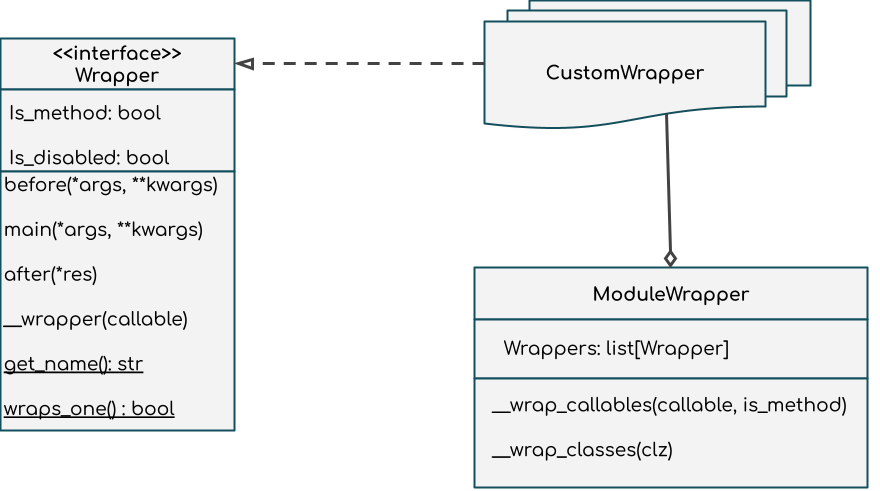
\includegraphics[width=0.6\textwidth]{src/pic/wrapper_uml.png}
\caption{The Wrapper interface: The Wrapper is the interface that controls the workflow of its derived classes. All \texttt{CustomWrapper} classes derived from the \texttt{Wrapper} may implement the \texttt{before, main} and \texttt{after} functions. The \texttt{\_\_wrapper} function is responsible for coordinating between the three main function and calling them in sequence. The static function \texttt{get\_name} specifies the target function or class in PyNEST, and finally the other static function \texttt{wraps\_one} indicates how many \texttt{Wrapper} instances should be created. Additionally, we have the \texttt{ModuleWrapper} that is responsible for creating the \texttt{CustomWrapper} instances and matching them with their target functions in PyNEST.}
\label{fig:wrapper_uml}
\end{figure}

As mentioned in the previous section, each \emph{Wrapper} object has three main functions to control the interception of the PyNEST calls. The \texttt{before()} function is responsible for preprocessing the input values that are given to the PyNEST function. Secondly, we have \texttt{main()}, which takes the modified parameters from the \texttt{before()} function and executes the real PyNEST function. Finally, we have the \texttt{after()} function that takes the output of the \texttt{main()} function and modifies it if necessary. On top of these core functions, we have two additional functions: \texttt{get\_name()} returns the name of the function that we want to wrap, and \texttt{wraps\_one()} indicates if this \texttt{Wrapper} object is wrapping a single or multiple functions. In case we wrap multiple functions, the \texttt{get\_name()} function must return a list containing the names of all wrapped functions. The function that brings all pieces together is \texttt{\_\_wrapper()}, which is responsible for calling \texttt{before()}, \texttt{main()} and \texttt{after()}.

The \texttt{ModuleWrapper} is responsible for matching the custom implemented wrappers with the targeted PyNEST objects. It iterates over all functions and classes and replaces them with their corresponding wrappers. finally, we have the \texttt{CustomWrappers} representing the derived classes from the \texttt{Wrapper} interface. Those derived classes can be seen in \autoref{fig:wrapper_derived}.

\subsection{The derived wrapper classes}

The \emph{Wrapper} interface on its own is not very useful for implementing the JIT mechanism, and it requires concrete implementations for each function we want to control. Each class derived from the \emph{Wrapper} interface wraps either a \emph{function} or a \emph{class} in PyNEST. In \autoref{fig:wrapper_derived}, we show all currently implemented wrappers. Most of them use a \texttt{helper} class that contains the required logic for making the JIT mechanism work. In the following, we list the implemented wrappers and discuss their usage.

\begin{figure}[ht!]
\centering


\tikzset{every picture/.style={line width=0.75pt}} %set default line width to 0.75pt
\scalebox{0.5}{
\begin{tikzpicture}[x=0.75pt,y=0.75pt,yscale=-1,xscale=1]
%uncomment if require: \path (0,519); %set diagram left start at 0, and has height of 519

%Rounded Rect [id:dp08332665529733485]
\draw  [color={rgb, 255:red, 139; green, 87; blue, 42 }  ,draw opacity=1 ][line width=2.25]  (277,217) .. controls (277,212.58) and (280.58,209) .. (285,209) -- (395.8,209) .. controls (400.22,209) and (403.8,212.58) .. (403.8,217) -- (403.8,241) .. controls (403.8,245.42) and (400.22,249) .. (395.8,249) -- (285,249) .. controls (280.58,249) and (277,245.42) .. (277,241) -- cycle ;
%Rounded Rect [id:dp643201073355989]
\draw  [color={rgb, 255:red, 139; green, 87; blue, 42 }  ,draw opacity=1 ][line width=2.25]  (1.8,427) .. controls (1.8,422.58) and (5.38,419) .. (9.8,419) -- (191.8,419) .. controls (196.22,419) and (199.8,422.58) .. (199.8,427) -- (199.8,451) .. controls (199.8,455.42) and (196.22,459) .. (191.8,459) -- (9.8,459) .. controls (5.38,459) and (1.8,455.42) .. (1.8,451) -- cycle ;
%Rounded Rect [id:dp9738213759503345]
\draw  [color={rgb, 255:red, 139; green, 87; blue, 42 }  ,draw opacity=1 ][line width=2.25]  (2.8,262) .. controls (2.8,257.58) and (6.38,254) .. (10.8,254) -- (136.8,254) .. controls (141.22,254) and (144.8,257.58) .. (144.8,262) -- (144.8,286) .. controls (144.8,290.42) and (141.22,294) .. (136.8,294) -- (10.8,294) .. controls (6.38,294) and (2.8,290.42) .. (2.8,286) -- cycle ;
%Rounded Rect [id:dp39360724795655755]
\draw  [color={rgb, 255:red, 139; green, 87; blue, 42 }  ,draw opacity=1 ][line width=2.25]  (503,349) .. controls (503,344.58) and (506.58,341) .. (511,341) -- (645.8,341) .. controls (650.22,341) and (653.8,344.58) .. (653.8,349) -- (653.8,373) .. controls (653.8,377.42) and (650.22,381) .. (645.8,381) -- (511,381) .. controls (506.58,381) and (503,377.42) .. (503,373) -- cycle ;
%Rounded Rect [id:dp2385264912044227]
\draw  [color={rgb, 255:red, 139; green, 87; blue, 42 }  ,draw opacity=1 ][line width=2.25]  (255.8,480) .. controls (255.8,475.58) and (259.38,472) .. (263.8,472) -- (444.8,472) .. controls (449.22,472) and (452.8,475.58) .. (452.8,480) -- (452.8,504) .. controls (452.8,508.42) and (449.22,512) .. (444.8,512) -- (263.8,512) .. controls (259.38,512) and (255.8,508.42) .. (255.8,504) -- cycle ;
%Rounded Rect [id:dp04455155996593918]
\draw  [color={rgb, 255:red, 139; green, 87; blue, 42 }  ,draw opacity=1 ][line width=2.25]  (153.8,33) .. controls (153.8,28.58) and (157.38,25) .. (161.8,25) -- (319.8,25) .. controls (324.22,25) and (327.8,28.58) .. (327.8,33) -- (327.8,57) .. controls (327.8,61.42) and (324.22,65) .. (319.8,65) -- (161.8,65) .. controls (157.38,65) and (153.8,61.42) .. (153.8,57) -- cycle ;
%Rounded Rect [id:dp5139694395821088]
\draw  [color={rgb, 255:red, 139; green, 87; blue, 42 }  ,draw opacity=1 ][line width=2.25]  (5.8,100) .. controls (5.8,95.58) and (9.38,92) .. (13.8,92) -- (137.8,92) .. controls (142.22,92) and (145.8,95.58) .. (145.8,100) -- (145.8,124) .. controls (145.8,128.42) and (142.22,132) .. (137.8,132) -- (13.8,132) .. controls (9.38,132) and (5.8,128.42) .. (5.8,124) -- cycle ;
%Rounded Rect [id:dp796653880823329]
\draw  [color={rgb, 255:red, 139; green, 87; blue, 42 }  ,draw opacity=1 ][line width=2.25]  (3.8,181) .. controls (3.8,176.58) and (7.38,173) .. (11.8,173) -- (129.8,173) .. controls (134.22,173) and (137.8,176.58) .. (137.8,181) -- (137.8,205) .. controls (137.8,209.42) and (134.22,213) .. (129.8,213) -- (11.8,213) .. controls (7.38,213) and (3.8,209.42) .. (3.8,205) -- cycle ;
%Rounded Rect [id:dp8115528255145159]
\draw  [color={rgb, 255:red, 139; green, 87; blue, 42 }  ,draw opacity=1 ][line width=2.25]  (1.8,349) .. controls (1.8,344.58) and (5.38,341) .. (9.8,341) -- (159.8,341) .. controls (164.22,341) and (167.8,344.58) .. (167.8,349) -- (167.8,373) .. controls (167.8,377.42) and (164.22,381) .. (159.8,381) -- (9.8,381) .. controls (5.38,381) and (1.8,377.42) .. (1.8,373) -- cycle ;
%Rounded Rect [id:dp6414618614909982]
\draw  [color={rgb, 255:red, 139; green, 87; blue, 42 }  ,draw opacity=1 ][line width=2.25]  (480.8,268) .. controls (480.8,263.58) and (484.38,260) .. (488.8,260) -- (645.8,260) .. controls (650.22,260) and (653.8,263.58) .. (653.8,268) -- (653.8,292) .. controls (653.8,296.42) and (650.22,300) .. (645.8,300) -- (488.8,300) .. controls (484.38,300) and (480.8,296.42) .. (480.8,292) -- cycle ;
%Rounded Rect [id:dp7381489249035267]
\draw  [color={rgb, 255:red, 139; green, 87; blue, 42 }  ,draw opacity=1 ][line width=2.25]  (485.8,182) .. controls (485.8,177.58) and (489.38,174) .. (493.8,174) -- (648.8,174) .. controls (653.22,174) and (656.8,177.58) .. (656.8,182) -- (656.8,206) .. controls (656.8,210.42) and (653.22,214) .. (648.8,214) -- (493.8,214) .. controls (489.38,214) and (485.8,210.42) .. (485.8,206) -- cycle ;
%Rounded Rect [id:dp704574691668346]
\draw  [color={rgb, 255:red, 139; green, 87; blue, 42 }  ,draw opacity=1 ][line width=2.25]  (476.8,102) .. controls (476.8,97.58) and (480.38,94) .. (484.8,94) -- (645.8,94) .. controls (650.22,94) and (653.8,97.58) .. (653.8,102) -- (653.8,126) .. controls (653.8,130.42) and (650.22,134) .. (645.8,134) -- (484.8,134) .. controls (480.38,134) and (476.8,130.42) .. (476.8,126) -- cycle ;
%Rounded Rect [id:dp33221553170106266]
\draw  [color={rgb, 255:red, 139; green, 87; blue, 42 }  ,draw opacity=1 ][line width=2.25]  (381.8,32) .. controls (381.8,27.58) and (385.38,24) .. (389.8,24) -- (547.8,24) .. controls (552.22,24) and (555.8,27.58) .. (555.8,32) -- (555.8,56) .. controls (555.8,60.42) and (552.22,64) .. (547.8,64) -- (389.8,64) .. controls (385.38,64) and (381.8,60.42) .. (381.8,56) -- cycle ;
%Rounded Rect [id:dp11416390733512127]
\draw  [color={rgb, 255:red, 139; green, 87; blue, 42 }  ,draw opacity=1 ][line width=2.25]  (499,425) .. controls (499,420.58) and (502.58,417) .. (507,417) -- (641.8,417) .. controls (646.22,417) and (649.8,420.58) .. (649.8,425) -- (649.8,449) .. controls (649.8,453.42) and (646.22,457) .. (641.8,457) -- (507,457) .. controls (502.58,457) and (499,453.42) .. (499,449) -- cycle ;
%Straight Lines [id:da7321475284754999]
\draw [line width=1.5]  [dash pattern={on 1.69pt off 2.76pt}]  (144.8,113.6) -- (273.85,214.54) ;
\draw [shift={(277,217)}, rotate = 218.03] [fill={rgb, 255:red, 0; green, 0; blue, 0 }  ][line width=0.08]  [draw opacity=0] (11.61,-5.58) -- (0,0) -- (11.61,5.58) -- cycle    ;
%Straight Lines [id:da826027105738447]
\draw [line width=1.5]  [dash pattern={on 1.69pt off 2.76pt}]  (141.8,191.6) -- (270.92,224.61) ;
\draw [shift={(274.8,225.6)}, rotate = 194.34] [fill={rgb, 255:red, 0; green, 0; blue, 0 }  ][line width=0.08]  [draw opacity=0] (11.61,-5.58) -- (0,0) -- (11.61,5.58) -- cycle    ;
%Straight Lines [id:da9419415019749295]
\draw [line width=1.5]  [dash pattern={on 1.69pt off 2.76pt}]  (144.8,272.6) -- (269.98,233.78) ;
\draw [shift={(273.8,232.6)}, rotate = 162.77] [fill={rgb, 255:red, 0; green, 0; blue, 0 }  ][line width=0.08]  [draw opacity=0] (11.61,-5.58) -- (0,0) -- (11.61,5.58) -- cycle    ;
%Straight Lines [id:da2009447559522246]
\draw [line width=1.5]  [dash pattern={on 1.69pt off 2.76pt}]  (169.8,364.6) -- (274.38,244.02) ;
\draw [shift={(277,241)}, rotate = 130.94] [fill={rgb, 255:red, 0; green, 0; blue, 0 }  ][line width=0.08]  [draw opacity=0] (11.61,-5.58) -- (0,0) -- (11.61,5.58) -- cycle    ;
%Curve Lines [id:da7600537285509692]
\draw [line width=1.5]  [dash pattern={on 1.69pt off 2.76pt}]  (191.8,419) .. controls (249.32,402.03) and (261.22,290.39) .. (298.85,255.16) ;
\draw [shift={(301.8,252.6)}, rotate = 141.34] [fill={rgb, 255:red, 0; green, 0; blue, 0 }  ][line width=0.08]  [draw opacity=0] (11.61,-5.58) -- (0,0) -- (11.61,5.58) -- cycle    ;
%Straight Lines [id:da1297385545876295]
\draw [line width=1.5]  [dash pattern={on 1.69pt off 2.76pt}]  (345.8,472.6) -- (341.09,255) ;
\draw [shift={(341,251)}, rotate = 88.76] [fill={rgb, 255:red, 0; green, 0; blue, 0 }  ][line width=0.08]  [draw opacity=0] (11.61,-5.58) -- (0,0) -- (11.61,5.58) -- cycle    ;
%Curve Lines [id:da8119155428391331]
\draw [line width=1.5]  [dash pattern={on 1.69pt off 2.76pt}]  (492.8,433.6) .. controls (470.6,411.4) and (399.99,291.43) .. (381.59,258.8) ;
\draw [shift={(379.8,255.6)}, rotate = 60.95] [fill={rgb, 255:red, 0; green, 0; blue, 0 }  ][line width=0.08]  [draw opacity=0] (11.61,-5.58) -- (0,0) -- (11.61,5.58) -- cycle    ;
%Straight Lines [id:da43888705895379454]
\draw [line width=1.5]  [dash pattern={on 1.69pt off 2.76pt}]  (500.8,367.6) -- (406.23,244.18) ;
\draw [shift={(403.8,241)}, rotate = 52.54] [fill={rgb, 255:red, 0; green, 0; blue, 0 }  ][line width=0.08]  [draw opacity=0] (11.61,-5.58) -- (0,0) -- (11.61,5.58) -- cycle    ;
%Straight Lines [id:da38095702214592175]
\draw [line width=1.5]  [dash pattern={on 1.69pt off 2.76pt}]  (479.8,274.6) -- (411.17,230.75) ;
\draw [shift={(407.8,228.6)}, rotate = 32.57] [fill={rgb, 255:red, 0; green, 0; blue, 0 }  ][line width=0.08]  [draw opacity=0] (11.61,-5.58) -- (0,0) -- (11.61,5.58) -- cycle    ;
%Straight Lines [id:da685328333847449]
\draw [line width=1.5]  [dash pattern={on 1.69pt off 2.76pt}]  (486.8,192.6) -- (407.64,215.87) ;
\draw [shift={(403.8,217)}, rotate = 343.62] [fill={rgb, 255:red, 0; green, 0; blue, 0 }  ][line width=0.08]  [draw opacity=0] (11.61,-5.58) -- (0,0) -- (11.61,5.58) -- cycle    ;
%Straight Lines [id:da09283567688019034]
\draw [line width=1.5]  [dash pattern={on 1.69pt off 2.76pt}]  (473.8,119.6) -- (398.43,205.99) ;
\draw [shift={(395.8,209)}, rotate = 311.1] [fill={rgb, 255:red, 0; green, 0; blue, 0 }  ][line width=0.08]  [draw opacity=0] (11.61,-5.58) -- (0,0) -- (11.61,5.58) -- cycle    ;
%Curve Lines [id:da7212396930412046]
\draw [line width=1.5]  [dash pattern={on 1.69pt off 2.76pt}]  (395.8,67.6) .. controls (378.34,64.69) and (399.46,164.34) .. (385.22,203.18) ;
\draw [shift={(383.8,206.6)}, rotate = 295.28] [fill={rgb, 255:red, 0; green, 0; blue, 0 }  ][line width=0.08]  [draw opacity=0] (11.61,-5.58) -- (0,0) -- (11.61,5.58) -- cycle    ;
%Straight Lines [id:da6247278152361431]
\draw [line width=1.5]  [dash pattern={on 1.69pt off 2.76pt}]  (241.8,68.6) -- (337.46,201.35) ;
\draw [shift={(339.8,204.6)}, rotate = 234.22] [fill={rgb, 255:red, 0; green, 0; blue, 0 }  ][line width=0.08]  [draw opacity=0] (11.61,-5.58) -- (0,0) -- (11.61,5.58) -- cycle    ;

% Text Node
\draw (311,229) node [anchor=north west][inner sep=0.75pt]   [align=left] {{\fontfamily{pcr}\selectfont \textcolor[rgb]{0.55,0.34,0.16}{\textbf{Wrapper}}}};
% Text Node
\draw (8,430) node [anchor=north west][inner sep=0.75pt]   [align=left] {{\fontfamily{pcr}\selectfont \textbf{\textcolor[rgb]{0.55,0.34,0.16}{NodeCollectionWrapper}}}};
% Text Node
\draw (8,265) node [anchor=north west][inner sep=0.75pt]   [align=left] {{\fontfamily{pcr}\selectfont \textbf{\textcolor[rgb]{0.55,0.34,0.16}{DisableNestFunc}}}};
% Text Node
\draw (509,352) node [anchor=north west][inner sep=0.75pt]   [align=left] {\textbf{\textcolor[rgb]{0.55,0.34,0.16}{{\fontfamily{pcr}\selectfont GetStatusWrapper}}}};
% Text Node
\draw (265,482.5) node [anchor=north west][inner sep=0.75pt]   [align=left] {\textbf{\textcolor[rgb]{0.55,0.34,0.16}{\textbf{GetConnectionWrapper}}}};
% Text Node
\draw (175,38) node [anchor=north west][inner sep=0.75pt]   [align=left] {{\fontfamily{pcr}\selectfont \textcolor[rgb]{0.55,0.34,0.16}{\textbf{ConnectWrapper}}}};
% Text Node
\draw (20,103) node [anchor=north west][inner sep=0.75pt]   [align=left] {{\fontfamily{pcr}\selectfont \textbf{\textcolor[rgb]{0.55,0.34,0.16}{CreateWrapper}}}};
% Text Node
\draw (23,184) node [anchor=north west][inner sep=0.75pt]   [align=left] {\textbf{\textcolor[rgb]{0.55,0.34,0.16}{{\fontfamily{pcr}\selectfont ModelWrapper}}}};
% Text Node
\draw (11,352) node [anchor=north west][inner sep=0.75pt]   [align=left] {{\fontfamily{pcr}\selectfont \textbf{\textcolor[rgb]{0.55,0.34,0.16}{SimulationWrapper}}}};
% Text Node
\draw (492.3,273) node [anchor=north west][inner sep=0.75pt]   [align=left] {{\fontfamily{pcr}\selectfont \textbf{\textcolor[rgb]{0.55,0.34,0.16}{RestKernelWrapper}}}};
% Text Node
\draw (491,186) node [anchor=north west][inner sep=0.75pt]   [align=left] {\textbf{\textcolor[rgb]{0.55,0.34,0.16}{{\fontfamily{pcr}\selectfont GetDefaultsWrapper}}}};
% Text Node
\draw (487,106) node [anchor=north west][inner sep=0.75pt]   [align=left] {\textbf{\textcolor[rgb]{0.55,0.34,0.16}{{\fontfamily{pcr}\selectfont SetDefaultsWrapper}}}};
% Text Node
\draw (398,37) node [anchor=north west][inner sep=0.75pt]   [align=left] {{\fontfamily{pcr}\selectfont \textcolor[rgb]{0.55,0.34,0.16}{\textbf{CopyModelWrapper}}}};
% Text Node
\draw (505,430) node [anchor=north west][inner sep=0.75pt]   [align=left] {\textbf{\textcolor[rgb]{0.55,0.34,0.16}{{\fontfamily{pcr}\selectfont SetStatusWrapper}}}};
% Text Node
\draw (285,213) node [anchor=north west][inner sep=0.75pt]   [align=left] {{\fontfamily{pcr}\selectfont \textcolor[rgb]{0.55,0.34,0.16}{≪interface≫}}};


\end{tikzpicture}
}
\caption{The implemented \texttt{CustomWrapper} classes derived from the \texttt{Wrapper} interface.}
\label{fig:wrapper_derived}
\end{figure}


\begin{description}
   \item[\mdseries\texttt{CreateWrapper}]: responsible for searching the model in the \emph{file system} and in the NestKernel built-in models and creating instances from it.
   \item[\mdseries\texttt{ConnectWrapper}]: responsible for making sure that we are always using the right model while calling the \texttt{Connect()} function. This may swap network elements under some conditions.
   \item[\mdseries\texttt{CopyModelWrapper}]: shares the functionality of the \texttt{CreateWrapper} for searching and installing the model in the NestKernel. In addition, it creates a copy of the found model.
   \item[\mdseries\texttt{SetStatusWrapper{\normalfont/}GetStatusWrapper}]: set/get the attributes of the model's instances.
   \item[\mdseries\texttt{SetDefaultWrapper{\normalfont/}GetDefaultWrapper}]: set/get the default values of the model. Even if the model is not yet registered in the NestKernel, the user can create instances of the copied model.
   \item[\mdseries\texttt{GetConnectionWrapper}]: returns the existing connections between source and target.
   \item[\mdseries\texttt{ResetKernelWrapper}]: resets the information about the models stored in the JIT related classes and calls the \texttt{ResetKerenel()} function.
   \item[\mdseries\texttt{NodeCollectionWrapper}]: returns an object containing the real object from the NestKernel and the JIT class instances.
   \item[\mdseries\texttt{ModelWrapper}]: returns all registered models from both the JIT related classes and NestKernel.
   \item[\mdseries\texttt{SimulationWrapper}]: makes sure that all JIT model instances are available in the NestKernel to start the simulation.
   \item[\mdseries\texttt{DisableNestFunc}]: skips the call of the PyNEST function.
\end{description}

   In the next step, we explain how to add a new wrapper to the JIT mechanism and explain the logic and execution flow behind the most important implemented wrappers. Here, the \texttt{CreateWrapper}, \texttt{ConnectWrapper} and \texttt{SimulateWrapper} are of most interest, the others follow the same logic.

\subsection{Adding a new wrapper class}

As shown in \autoref{lst:custom_wrapper}, wrapping a new function or class in PyNEST is very simple. We only need to add the new implementation to the \texttt{wrapper.py} Python file containing all implemented wrappers. At this point, there are no restrictions to how the \texttt{before()}/\texttt{main()}/\texttt{after()} functions must be implemented. The implemented wrapper has complete control on how the target PyNEST function should behave with respect to the JIT mechanism.

\begin{figure}[ht!]
\centering
 \begin{lstlisting}[language=Python, label=lst:custom_wrapper, caption={CustomWrapper example}]
from jit.wrapper.wrapper import Wrapper

class CustomWrapper(Wrapper):
    def __init__(self, nest_func):
        super.__init__(nest_func, is_method=False, is_disabled=False)
    def __process_input(self, *args, **kwargs):
        # do something with the input
        return args, kwargs
    def __process_output(self, *res):
        # do something with the output
        return res
    def before(self, *args, **kwargs):
        return self.__process_input(args, kwargs)
    def main(self, *args, **kwargs):
        return self.nest_func(args, kwargs)
    def after(self, *res):
        return self.__process_output(res)
    @staticmethod
    def get_name():
        return "nest.{func_name}"
    @staticmethod
    def wraps_one():
        return True
\end{lstlisting}
    %\caption{CustomWrapper example}
    %\label{fig:custom_wrapper}
\end{figure}


It is important to note here that the developer of a wrapper does not have to provide implementations of \texttt{before()}, \texttt{main()} and \texttt{after()} as the base class already contains useful defaults: the default behavior of the \texttt{before()} function is to just return the input parameters unchanged, the \texttt{main()} function calls the real PyNEST function and the \texttt{after()} function checks if \texttt{main()} has returned anything and returns the same object unchanged, or nothing if \texttt{main()} did not return anything.

Custom \emph{Wrapper}s are registrered automatically upon importing the JIT module in the Python script. In the \texttt{wrappers.py} file, we have the \texttt{install\_wrappers()} function shown in \autoref{lst:wrapper_reg} that is responsible for iterating over all subclasses implementing the \texttt{Wrapper} interface and inserting them into a dictionary, having as \emph{key} the target function name and as \emph{value} the derived wrapper class. The \texttt{ModuleWrapper} then imports the dictionary and iterates over its keys, comparing them with PyNEST functions and classes. Once a match is found, the \texttt{ModuleWrapper} creates an instance of the \texttt{CustomWrapper} and extends the JIT module with a new function or class having the same name as the one coming from the PyNEST module. The new inserted functions or classes in JIT are either the original ones or an instance of the \texttt{CustomWrapper}.

\begin{figure}[ht!]
    \centering
    \begin{lstlisting}[language=Python, label=lst:wrapper_reg, caption={Registering Wrappers}]
def install_wrappers():
    sub_classes = Wrapper.__subclasses__()
    to_wrap = {}
    for sub_clz in sub_classes:
        if sub_clz.wrapps_one():
            to_wrap[sub_clz.get_name()] = sub_clz
        else:
            for name in sub_clz.get_name():
                to_wrap[name] = sub_clz
    return to_wrap
\end{lstlisting}
    %\caption{Registering Wrappers}
    %\label{fig:wrapper_reg}
\end{figure}

\section{Wrapping PyNEST: the \texttt{Create()} function}

New model instances in PyNEST are created by calling the \texttt{Create()} function, which takes four parameters. The first is the name of the model, the second is the number of instances we want to create, the third are parameters for the new instances and the is for indicating the spatial distribution of the created nodes. The return value of the function is a \texttt{NodeCollection} object, which is a compact and contiguous representation of the created nodes on the Python side. Internally, the \texttt{NodeCollection} object stores only the first and last ID of a continuous space of nodes or a concatenation of such structures. If we create $n=10$ instances of a model and only select the odd (or even) positions, the \texttt{NodeCollection} object will have five blocks pointing to the individual odd/even positions. \autoref{fig:node_collection} shows an example of how the \texttt{NodeCollection} may look like. At the start, we have only a single block containing the first and last ID of the nodes. By splitting the created \texttt{NodeCollection} into even and odd IDs, we get two \texttt{NodeCollection} objects, each with five blocks. Each of these blocks contains only a single ID.

\begin{figure}[ht!]
\centering
\tikzset{every picture/.style={line width=0.75pt}} %set default line width to 0.75pt
\scalebox{0.5}{
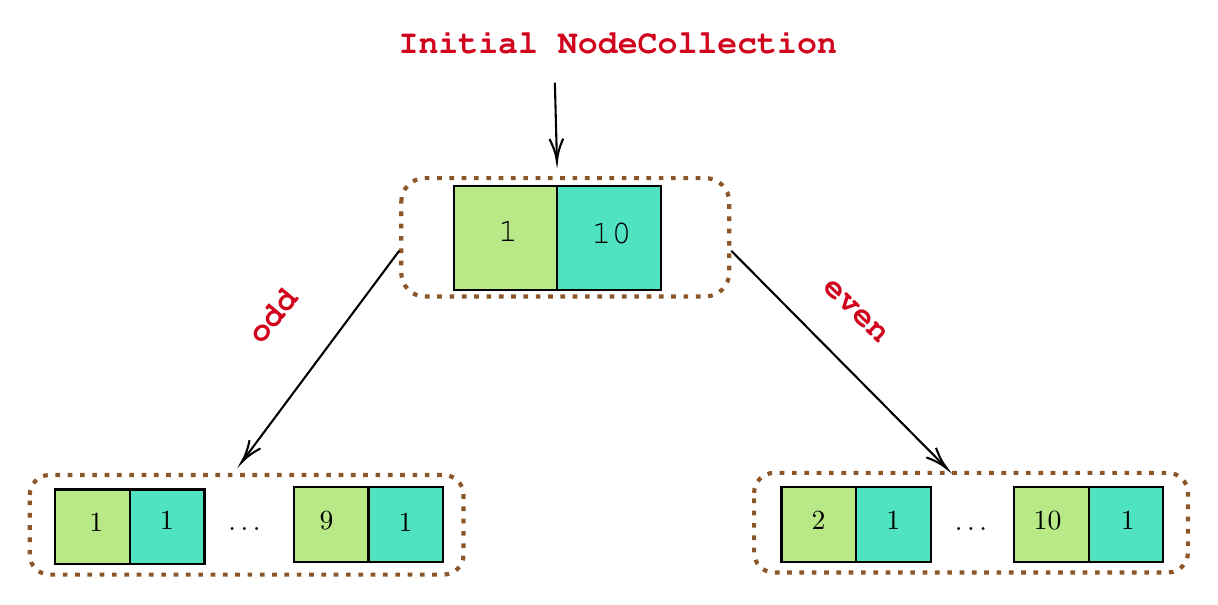
\begin{tikzpicture}[x=0.75pt,y=0.75pt,yscale=-1,xscale=1]
%uncomment if require: \path (0,420); %set diagram left start at 0, and has height of 420

%Shape: Square [id:dp14505338419362657]
\draw  [fill={rgb, 255:red, 184; green, 233; blue, 134 }  ,fill opacity=1 ] (283,86) -- (333,86) -- (333,136) -- (283,136) -- cycle ;
%Shape: Square [id:dp5690214325454108]
\draw  [fill={rgb, 255:red, 80; green, 227; blue, 194 }  ,fill opacity=1 ] (333,86) -- (383,86) -- (383,136) -- (333,136) -- cycle ;
%Rounded Rect [id:dp8563434876650051]
\draw  [color={rgb, 255:red, 139; green, 87; blue, 42 }  ,draw opacity=1 ][dash pattern={on 1.69pt off 2.76pt}][line width=1.5]  (257.8,93.4) .. controls (257.8,87.1) and (262.9,82) .. (269.2,82) -- (404.4,82) .. controls (410.7,82) and (415.8,87.1) .. (415.8,93.4) -- (415.8,127.6) .. controls (415.8,133.9) and (410.7,139) .. (404.4,139) -- (269.2,139) .. controls (262.9,139) and (257.8,133.9) .. (257.8,127.6) -- cycle ;
%Shape: Square [id:dp7833262911739212]
\draw  [fill={rgb, 255:red, 184; green, 233; blue, 134 }  ,fill opacity=1 ] (206,231) -- (242,231) -- (242,267) -- (206,267) -- cycle ;
%Shape: Square [id:dp9953924667288327]
\draw  [fill={rgb, 255:red, 80; green, 227; blue, 194 }  ,fill opacity=1 ] (242,231) -- (278,231) -- (278,267) -- (242,267) -- cycle ;
%Shape: Square [id:dp6299533126736598]
\draw  [fill={rgb, 255:red, 184; green, 233; blue, 134 }  ,fill opacity=1 ] (91,232) -- (127,232) -- (127,268) -- (91,268) -- cycle ;
%Shape: Square [id:dp19915315419671153]
\draw  [fill={rgb, 255:red, 80; green, 227; blue, 194 }  ,fill opacity=1 ] (127,232) -- (163,232) -- (163,268) -- (127,268) -- cycle ;
%Shape: Square [id:dp5267204094552598]
\draw  [fill={rgb, 255:red, 184; green, 233; blue, 134 }  ,fill opacity=1 ] (441,231) -- (477,231) -- (477,267) -- (441,267) -- cycle ;
%Shape: Square [id:dp7392648786591738]
\draw  [fill={rgb, 255:red, 80; green, 227; blue, 194 }  ,fill opacity=1 ] (477,231) -- (513,231) -- (513,267) -- (477,267) -- cycle ;
%Shape: Square [id:dp2621212093475398]
\draw  [fill={rgb, 255:red, 184; green, 233; blue, 134 }  ,fill opacity=1 ] (553,231) -- (589,231) -- (589,267) -- (553,267) -- cycle ;
%Shape: Square [id:dp328789805802878]
\draw  [fill={rgb, 255:red, 80; green, 227; blue, 194 }  ,fill opacity=1 ] (589,231) -- (625,231) -- (625,267) -- (589,267) -- cycle ;
%Straight Lines [id:da7176298813855051]
\draw    (331.8,36) -- (332.75,72) ;
\draw [shift={(332.8,74)}, rotate = 268.49] [color={rgb, 255:red, 0; green, 0; blue, 0 }  ][line width=0.75]    (10.93,-3.29) .. controls (6.95,-1.4) and (3.31,-0.3) .. (0,0) .. controls (3.31,0.3) and (6.95,1.4) .. (10.93,3.29)   ;
%Rounded Rect [id:dp5333242873793238]
\draw  [color={rgb, 255:red, 139; green, 87; blue, 42 }  ,draw opacity=1 ][dash pattern={on 1.69pt off 2.76pt}][line width=1.5]  (78.8,234.6) .. controls (78.8,229.3) and (83.1,225) .. (88.4,225) -- (278.2,225) .. controls (283.5,225) and (287.8,229.3) .. (287.8,234.6) -- (287.8,263.4) .. controls (287.8,268.7) and (283.5,273) .. (278.2,273) -- (88.4,273) .. controls (83.1,273) and (78.8,268.7) .. (78.8,263.4) -- cycle ;
%Rounded Rect [id:dp9183238991512817]
\draw  [color={rgb, 255:red, 139; green, 87; blue, 42 }  ,draw opacity=1 ][dash pattern={on 1.69pt off 2.76pt}][line width=1.5]  (427.8,233.6) .. controls (427.8,228.3) and (432.1,224) .. (437.4,224) -- (627.2,224) .. controls (632.5,224) and (636.8,228.3) .. (636.8,233.6) -- (636.8,262.4) .. controls (636.8,267.7) and (632.5,272) .. (627.2,272) -- (437.4,272) .. controls (432.1,272) and (427.8,267.7) .. (427.8,262.4) -- cycle ;
%Straight Lines [id:da22871011626744342]
\draw    (256.8,117) -- (181.99,217.4) ;
\draw [shift={(180.8,219)}, rotate = 306.69] [color={rgb, 255:red, 0; green, 0; blue, 0 }  ][line width=0.75]    (10.93,-3.29) .. controls (6.95,-1.4) and (3.31,-0.3) .. (0,0) .. controls (3.31,0.3) and (6.95,1.4) .. (10.93,3.29)   ;
%Straight Lines [id:da2777097984312962]
\draw    (416.8,117) -- (519.39,220.58) ;
\draw [shift={(520.8,222)}, rotate = 225.27] [color={rgb, 255:red, 0; green, 0; blue, 0 }  ][line width=0.75]    (10.93,-3.29) .. controls (6.95,-1.4) and (3.31,-0.3) .. (0,0) .. controls (3.31,0.3) and (6.95,1.4) .. (10.93,3.29)   ;
%Shape: Square [id:dp3719120065205612]
\draw  [color={rgb, 255:red, 255; green, 255; blue, 255 }  ,draw opacity=1 ][fill={rgb, 255:red, 255; green, 255; blue, 255 }  ,fill opacity=1 ] (519.3,235) -- (545.3,235) -- (545.3,261) -- (519.3,261) -- cycle ;
%Shape: Square [id:dp3898179761369387]
\draw  [color={rgb, 255:red, 255; green, 255; blue, 255 }  ,draw opacity=1 ][fill={rgb, 255:red, 255; green, 255; blue, 255 }  ,fill opacity=1 ] (170.3,236) -- (196.3,236) -- (196.3,262) -- (170.3,262) -- cycle ;

% Text Node
\draw (303,101) node [anchor=north west][inner sep=0.75pt]   [align=left] {{\fontfamily{pcr}\selectfont {\large 1}}};
% Text Node
\draw (348,102) node [anchor=north west][inner sep=0.75pt]   [align=left] {{\fontfamily{pcr}\selectfont {\large 10}}};
% Text Node
\draw (255,10) node [anchor=north west][inner sep=0.75pt]   [align=left] {{\fontfamily{pcr}\selectfont {\large \textcolor[rgb]{0.82,0.01,0.11}{\textbf{Initial NodeCollection}}}}};
% Text Node
\draw (106,242) node [anchor=north west][inner sep=0.75pt]   [align=left] {1};
% Text Node
\draw (140,241) node [anchor=north west][inner sep=0.75pt]   [align=left] {1};
% Text Node
\draw (454,241) node [anchor=north west][inner sep=0.75pt]   [align=left] {2};
% Text Node
\draw (490,241) node [anchor=north west][inner sep=0.75pt]   [align=left] {1};
% Text Node
\draw (603,241) node [anchor=north west][inner sep=0.75pt]   [align=left] {1};
% Text Node
\draw (217,241) node [anchor=north west][inner sep=0.75pt]   [align=left] {9};
% Text Node
\draw (255,242) node [anchor=north west][inner sep=0.75pt]   [align=left] {1};
% Text Node
\draw (561,241) node [anchor=north west][inner sep=0.75pt]   [align=left] {10};
% Text Node
\draw (180.34,156.35) node [anchor=north west][inner sep=0.75pt]  [rotate=-309.65] [align=left] {{\fontfamily{pcr}\selectfont {\large \textcolor[rgb]{0.82,0.01,0.11}{\textbf{odd}}}}};
% Text Node
\draw (465.4,128.02) node [anchor=north west][inner sep=0.75pt]  [rotate=-44.1] [align=left] {{\fontfamily{pcr}\selectfont {\large \textcolor[rgb]{0.82,0.01,0.11}{\textbf{even}}}}};
% Text Node
\draw (523,249) node [anchor=north west][inner sep=0.75pt]   [align=left] {\dots};
% Text Node
\draw (173,249) node [anchor=north west][inner sep=0.75pt]   [align=left] {\dots};


\end{tikzpicture}
}
\caption{Splitting a \texttt{NodeCollection} object: The initial \texttt{NodeCollection} instance has ten items. Instead of storing all ten items individually, the \texttt{NodeCollection} stores only the first and the last ID in the collection. Splitting the \texttt{NodeCollection} into even and odd IDs, we get two \texttt{NodeCollection} objects, each having five items. The separation of IDs in each split is due to non-contiguous space between them. \texttt{NodeCollection}s with only a single element store the ID and their size of 1 instead of the last ID, hence the 1 in the final block of each of the \texttt{NodeCollection}s on the bottom.}
\label{fig:node_collection}
\end{figure}


In contrast to the initial block, the new blocks only store the ID of the first element and the size of 1. In case the slicing operation would result in larger blocks, they would have the same structure as the original block. It is important to note here that the size of the \texttt{NodeCollection} object is computed by summing the individual sizes of each block. Thus, the size of the original \texttt{NodeCollection} instance is not one, but instead is $last - first + 1 = 10 - 1 + 1 = 10$.

As depicted in \autoref{fig:node_collection_agg}, aggregating \texttt{NodeCollection} objects results in having the original \texttt{NodeCollection} instance. The logic behind the aggregation is to first sort everything by ID, then aggregate the IDs by the model they belong to, merge them into blocks and finally split these blocks into contiguous spaces.

\begin{figure}[ht!]
\centering

  \tikzset{every picture/.style={line width=0.75pt}} %set default line width to 0.75pt
  \scalebox{0.5}{
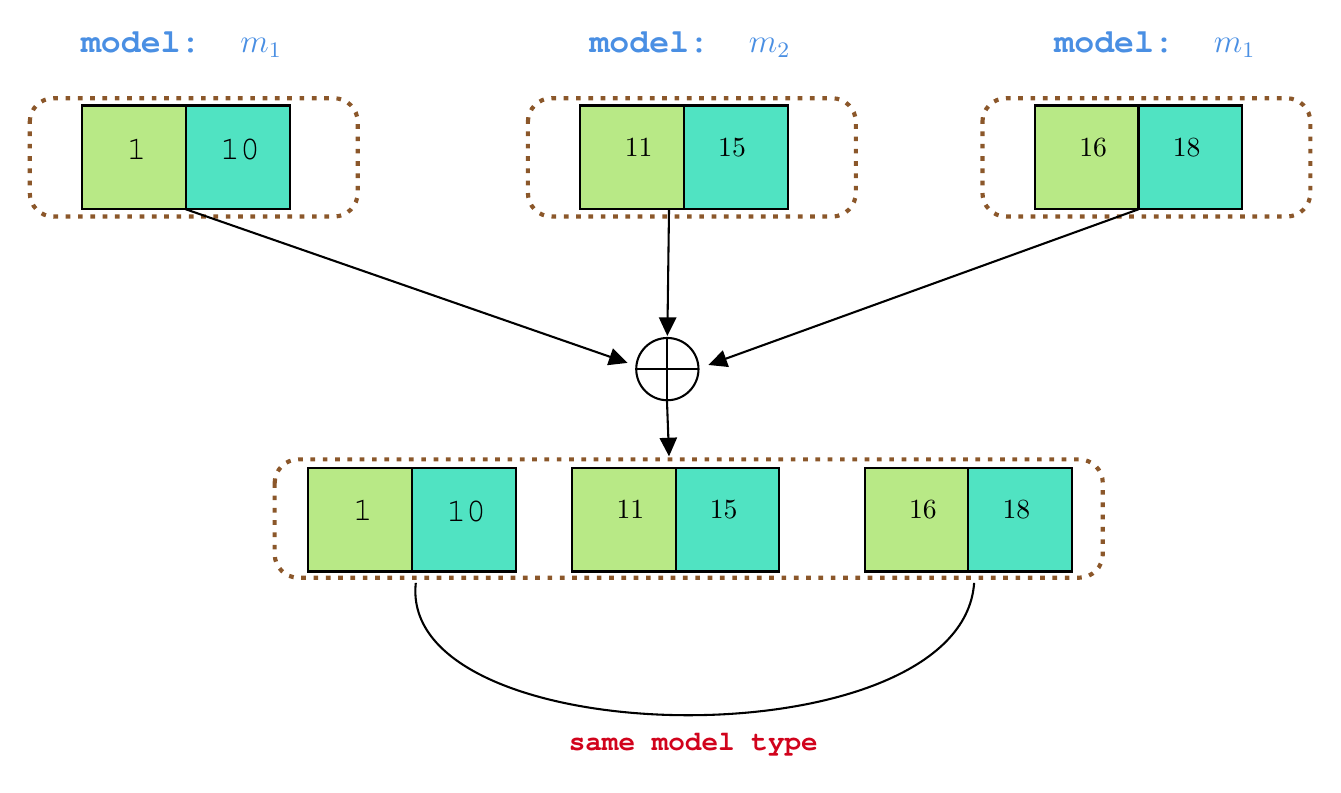
\begin{tikzpicture}[x=0.75pt,y=0.75pt,yscale=-1,xscale=1]
%uncomment if require: \path (0,420); %set diagram left start at 0, and has height of 420

%Shape: Square [id:dp847004206398758]
\draw  [fill={rgb, 255:red, 184; green, 233; blue, 134 }  ,fill opacity=1 ] (41,42) -- (91,42) -- (91,92) -- (41,92) -- cycle ;
%Shape: Square [id:dp7413686977322151]
\draw  [fill={rgb, 255:red, 80; green, 227; blue, 194 }  ,fill opacity=1 ] (91,42) -- (141,42) -- (141,92) -- (91,92) -- cycle ;
%Rounded Rect [id:dp9157715511667133]
\draw  [color={rgb, 255:red, 139; green, 87; blue, 42 }  ,draw opacity=1 ][dash pattern={on 1.69pt off 2.76pt}][line width=1.5]  (15.8,49.9) .. controls (15.8,43.6) and (20.9,38.5) .. (27.2,38.5) -- (162.4,38.5) .. controls (168.7,38.5) and (173.8,43.6) .. (173.8,49.9) -- (173.8,84.1) .. controls (173.8,90.4) and (168.7,95.5) .. (162.4,95.5) -- (27.2,95.5) .. controls (20.9,95.5) and (15.8,90.4) .. (15.8,84.1) -- cycle ;
%Shape: Square [id:dp7126705161517422]
\draw  [fill={rgb, 255:red, 184; green, 233; blue, 134 }  ,fill opacity=1 ] (281,42) -- (331,42) -- (331,92) -- (281,92) -- cycle ;
%Shape: Square [id:dp6046869167773221]
\draw  [fill={rgb, 255:red, 80; green, 227; blue, 194 }  ,fill opacity=1 ] (331,42) -- (381,42) -- (381,92) -- (331,92) -- cycle ;
%Rounded Rect [id:dp7623925132527456]
\draw  [color={rgb, 255:red, 139; green, 87; blue, 42 }  ,draw opacity=1 ][dash pattern={on 1.69pt off 2.76pt}][line width=1.5]  (255.8,49.9) .. controls (255.8,43.6) and (260.9,38.5) .. (267.2,38.5) -- (402.4,38.5) .. controls (408.7,38.5) and (413.8,43.6) .. (413.8,49.9) -- (413.8,84.1) .. controls (413.8,90.4) and (408.7,95.5) .. (402.4,95.5) -- (267.2,95.5) .. controls (260.9,95.5) and (255.8,90.4) .. (255.8,84.1) -- cycle ;
%Shape: Square [id:dp23969321871465432]
\draw  [fill={rgb, 255:red, 184; green, 233; blue, 134 }  ,fill opacity=1 ] (500,42) -- (550,42) -- (550,92) -- (500,92) -- cycle ;
%Shape: Square [id:dp5973854844810629]
\draw  [fill={rgb, 255:red, 80; green, 227; blue, 194 }  ,fill opacity=1 ] (550,42) -- (600,42) -- (600,92) -- (550,92) -- cycle ;
%Rounded Rect [id:dp4358433234191832]
\draw  [color={rgb, 255:red, 139; green, 87; blue, 42 }  ,draw opacity=1 ][dash pattern={on 1.69pt off 2.76pt}][line width=1.5]  (474.8,49.9) .. controls (474.8,43.6) and (479.9,38.5) .. (486.2,38.5) -- (621.4,38.5) .. controls (627.7,38.5) and (632.8,43.6) .. (632.8,49.9) -- (632.8,84.1) .. controls (632.8,90.4) and (627.7,95.5) .. (621.4,95.5) -- (486.2,95.5) .. controls (479.9,95.5) and (474.8,90.4) .. (474.8,84.1) -- cycle ;
%Shape: Square [id:dp6913149663475422]
\draw  [fill={rgb, 255:red, 184; green, 233; blue, 134 }  ,fill opacity=1 ] (150,216.5) -- (200,216.5) -- (200,266.5) -- (150,266.5) -- cycle ;
%Shape: Square [id:dp9939502562728053]
\draw  [fill={rgb, 255:red, 80; green, 227; blue, 194 }  ,fill opacity=1 ] (200,216.5) -- (250,216.5) -- (250,266.5) -- (200,266.5) -- cycle ;
%Rounded Rect [id:dp2894941589728419]
\draw  [color={rgb, 255:red, 139; green, 87; blue, 42 }  ,draw opacity=1 ][dash pattern={on 1.69pt off 2.76pt}][line width=1.5]  (133.8,223.9) .. controls (133.8,217.6) and (138.9,212.5) .. (145.2,212.5) -- (521.4,212.5) .. controls (527.7,212.5) and (532.8,217.6) .. (532.8,223.9) -- (532.8,258.1) .. controls (532.8,264.4) and (527.7,269.5) .. (521.4,269.5) -- (145.2,269.5) .. controls (138.9,269.5) and (133.8,264.4) .. (133.8,258.1) -- cycle ;
%Shape: Square [id:dp6685853677708664]
\draw  [fill={rgb, 255:red, 184; green, 233; blue, 134 }  ,fill opacity=1 ] (277,216.5) -- (327,216.5) -- (327,266.5) -- (277,266.5) -- cycle ;
%Shape: Square [id:dp4147175960535616]
\draw  [fill={rgb, 255:red, 80; green, 227; blue, 194 }  ,fill opacity=1 ] (327,216.5) -- (377,216.5) -- (377,266.5) -- (327,266.5) -- cycle ;
%Shape: Square [id:dp512011435333084]
\draw  [fill={rgb, 255:red, 184; green, 233; blue, 134 }  ,fill opacity=1 ] (418,216.5) -- (468,216.5) -- (468,266.5) -- (418,266.5) -- cycle ;
%Shape: Square [id:dp4778634283532628]
\draw  [fill={rgb, 255:red, 80; green, 227; blue, 194 }  ,fill opacity=1 ] (468,216.5) -- (518,216.5) -- (518,266.5) -- (468,266.5) -- cycle ;
%Straight Lines [id:da2340156449095352]
\draw [line width=0.75]    (91,92) -- (300.97,165.01) ;
\draw [shift={(303.8,166)}, rotate = 199.17] [fill={rgb, 255:red, 0; green, 0; blue, 0 }  ][line width=0.08]  [draw opacity=0] (8.93,-4.29) -- (0,0) -- (8.93,4.29) -- cycle    ;
%Straight Lines [id:da9639225095005677]
\draw    (323.8,92) -- (323.04,150) ;
\draw [shift={(323,153)}, rotate = 270.75] [fill={rgb, 255:red, 0; green, 0; blue, 0 }  ][line width=0.08]  [draw opacity=0] (8.93,-4.29) -- (0,0) -- (8.93,4.29) -- cycle    ;
%Straight Lines [id:da2987801737891538]
\draw    (550,92) -- (345.62,165.98) ;
\draw [shift={(342.8,167)}, rotate = 340.1] [fill={rgb, 255:red, 0; green, 0; blue, 0 }  ][line width=0.08]  [draw opacity=0] (8.93,-4.29) -- (0,0) -- (8.93,4.29) -- cycle    ;
\draw   (308,169) .. controls (308,160.72) and (314.72,154) .. (323,154) .. controls (331.28,154) and (338,160.72) .. (338,169) .. controls (338,177.28) and (331.28,184) .. (323,184) .. controls (314.72,184) and (308,177.28) .. (308,169) -- cycle ; \draw   (308,169) -- (338,169) ; \draw   (323,154) -- (323,184) ;
%Straight Lines [id:da9446189905883726]
\draw    (322.8,184) -- (323.69,208) ;
\draw [shift={(323.8,211)}, rotate = 267.88] [fill={rgb, 255:red, 0; green, 0; blue, 0 }  ][line width=0.08]  [draw opacity=0] (8.93,-4.29) -- (0,0) -- (8.93,4.29) -- cycle    ;
%Shape: Boxed Bezier Curve [id:dp5511245545993457]
\draw    (201.8,272) .. controls (192.8,355) and (464.8,359) .. (470.8,272) ;

% Text Node
\draw (61,56.5) node [anchor=north west][inner sep=0.75pt]   [align=left] {{\fontfamily{pcr}\selectfont {\large 1}}};
% Text Node
\draw (106,56.5) node [anchor=north west][inner sep=0.75pt]   [align=left] {{\fontfamily{pcr}\selectfont {\large 10}}};
% Text Node
\draw (301,56.5) node [anchor=north west][inner sep=0.75pt]   [align=left] {11};
% Text Node
\draw (346,56.5) node [anchor=north west][inner sep=0.75pt]   [align=left] {15};
% Text Node
\draw (520,56.5) node [anchor=north west][inner sep=0.75pt]   [align=left] {16};
% Text Node
\draw (565,56.5) node [anchor=north west][inner sep=0.75pt]   [align=left] {18};
% Text Node
\draw (284,5) node [anchor=north west][inner sep=0.75pt]   [align=left] {{\fontfamily{pcr}\selectfont {\large \textbf{\textcolor[rgb]{0.29,0.56,0.89}{model: $m_2$}}}}};
% Text Node
\draw (508,5) node [anchor=north west][inner sep=0.75pt]   [align=left] {{\fontfamily{pcr}\selectfont {\large \textcolor[rgb]{0.29,0.56,0.89}{\textbf{model: $m_1$}}}}};
% Text Node
\draw (39,5) node [anchor=north west][inner sep=0.75pt]   [align=left] {{\fontfamily{pcr}\selectfont {\large \textcolor[rgb]{0.29,0.56,0.89}{\textbf{model: $m_1$}}}}};
% Text Node
\draw (170,230.5) node [anchor=north west][inner sep=0.75pt]   [align=left] {{\fontfamily{pcr}\selectfont {\large 1}}};
% Text Node
\draw (215,231) node [anchor=north west][inner sep=0.75pt]   [align=left] {{\fontfamily{pcr}\selectfont {\large 10}}};
% Text Node
\draw (297,231) node [anchor=north west][inner sep=0.75pt]   [align=left] {11};
% Text Node
\draw (342,231) node [anchor=north west][inner sep=0.75pt]   [align=left] {15};
% Text Node
\draw (438,231) node [anchor=north west][inner sep=0.75pt]   [align=left] {16};
% Text Node
\draw (483,231) node [anchor=north west][inner sep=0.75pt]   [align=left] {18};
% Text Node
\draw (274,343) node [anchor=north west][inner sep=0.75pt]   [align=left] {\textcolor[rgb]{0.82,0.01,0.11}{{\fontfamily{pcr}\selectfont \textbf{same model type}}}};


\end{tikzpicture}
}
\caption{Aggregation of \texttt{NodeCollection} objects: We start with two models $m_1$ and $m_2$. The first model $m_1$ has two \texttt{NodeCollection} objects pointing to it. The first collection has ten items with IDs between 1 and 10, the second collection has only three items with IDs between 16 and 18. The second model $m_2$ has only one collection with five elements with IDs between 11 and 15. The aggregation of the three \texttt{NodeCollection} instances results in one \texttt{NodeCollection} object that handles the items as a single list, but also keeps the separation between the models and their IDs. }
\label{fig:node_collection_agg}
\end{figure}

A pre-condition for the \texttt{Create()} function to work and to return an instance of the \texttt{NodeCollection} object is to have the \emph{model} registered in the NestKernel (see \autoref{chap:funds}). The desired model is either already installed as a \emph{built-in} model in the NestKernel or it must be manually installed by first running the code generation pipeline and calling \texttt{Install()}. These steps must be carried out manually and repeatedly in any simulation script that uses an \emph{external} model that is not already available in the NestKernel. To automate this process, the \texttt{Create()} function must know in advance where to find the given model, register it and make it available for use without the user explicitly calling the code generator and the \texttt{Install()} function. To this end, we have the \texttt{CreateWrapper}, which exactly solves the problem by preparing everything automatically before calling the original \texttt{Create()} function. In the following subsection, we will discuss the \texttt{CreateWrapper} and discuss all important logic consideration to make it work correctly.

In \autoref{fig:pynestml_workflow} in \autoref{chap:funds}, we have split the code generation process into three steps. The parsing and validation, the transformation and finally the code generation and building the extension module. The simulation script can be split into three phases as well. At first, we have to create the nodes and, depending on the simulation scenario, parametrize them from random distributions, so the user can inspect the drawn values and apply some pre-analysis to the state of these nodes. Second, once the nodes are ready, we proceed to the next step and connect the nodes and create the network. Similarly to the nodes, the network can be a \emph{random network}, where nodes are connected with probability $p$, or connection parameters can be drawn from random distributions. Once the network is set and the random parameters are drawn, the user can inspect the topology of the network. The last step in the simulation script is to run the \texttt{Simulate()} function and wait for the simulation to finish. Afterwards the user can analyze the behavior of the network and check the final state of the nodes. It is important to mention that the configuration of the nodes and the network are two separate things, and they do not influence each other. The \texttt{CreateWrapper} makes use of this separation by splitting the code generation pipeline into two steps. The first step uses only the parsing and the transformation steps, whereas the code generation and building the extension module is executed in the background and the \texttt{Create()} function will not wait for the complete code generation pipeline to finish.

The main tasks for the \texttt{CreateWrapper} are thus to search for the specified model in the \emph{built-in} models, in the existing folders of the built libraries and finally in the folders containing the \texttt{.nestml} files. If the model is a \emph{built-in} model, the \texttt{CreateWrapper} simply calls \texttt{Create()} with the provided parameters. If the model already exists in one of the external libraries, the wrapper calls the \texttt{Install()} function to load the model and then calls \texttt{Create()}. In the most complicated scenario, the model's library does not exist, and therefore the code generation pipeline must be executed. It is important here to recall that when we reach the transformation phase, we generate a \emph{lightweight} version of the model by extracting its parameters and states and making them directly available after the call to \texttt{Create()} without waiting for the code generation and building, which takes place in a background process. Only the \texttt{Connect()} and \texttt{Simulate()} functions have to check the status of the running background process and on success the complete model will be registered, and it will become fully available for use.

In order for the \texttt{CreateWrapper} to hide all these steps for making the model available after the call to \texttt{Create()}, we need to have a class similar to the \texttt{NodeCollection} that works on the \emph{lightweight} version of the model. The name of this class is \texttt{NodeCollectionProxy}, and it will be explained later in this section. Along with this new class, the \texttt{CreateWrapper} uses a helper class called \texttt{CreateHelper} that takes responsibility for searching for the model and making it either completely or partially ready to query and to modify. All these components will be discussed in the following subsections.

\subsection{The \texttt{CreateWrapper}}

Due to the simplicity of the \texttt{Wrapper} interface, the \texttt{CreateWrapper} as depicted in \autoref{lst:create_wrapper} can be implemented by only using the \texttt{CreateHelper} that encapsulates the full logic behind the JIT-enabled \texttt{Create()} function. The \texttt{CreateHelper} provides a \texttt{Create()} function that has the same signature as the one of PyNEST, but instead of returning a \texttt{NodeCollection} object, it returns a \texttt{NodeCollectionProxy} object. The \texttt{before} function only stores the \texttt{NodeCollectionProxy} as a member object of the \texttt{CreateWrapper} class. As the \texttt{main()} function is not doing anything, the \texttt{before()} function just returns an empty tuple and an empty dictionary and the \texttt{after()} function simply returns the stored \texttt{NodeCollectionProxy} object, but does not have to do anything else.

\begin{figure}[ht!]
    \centering
    \begin{lstlisting}[language=Python, label=lst:create_wrapper, caption={The \texttt{CreateWrapper}}]
from jit.helpers.create_helper import CreateHelper
from jit.wrapper.wrapper import Wrapper

class CreateWrapper(Wrapper):
    def __init__(self, func):
        super().__init__(func, is_method=False, is_disabled=False)
        self.nodeCollectionProxy = None
    def before(self, model_name, n=1, params=None, positions=None):
        createHelper = CreateHelper()
        self.nodeCollectionProxy = createHelper.Create(
                                   model_name, n, params, positions)
        return (), {}
    def main(self, *args, **kwargs):
        pass
    def after(self, *res):
        return self.nodeCollectionProxy
    @staticmethod
    def get_name():
        return "nest.Create"
\end{lstlisting}
    %\caption{}
    %\label{fig:create_wrapper}
\end{figure}

\subsection{The \texttt{CreateHelper}}

The \texttt{CreateHelper} is responsble for controlling the full workflow of the \texttt{Create()} function. In order to understand the actions performed within each of the functions in \autoref{lst:create_helper}, we first need to understand the role of each of the \texttt{import}s. The first line imports the \texttt{ModelQuery} object, which is used to find the model and returns a handle that knows if the model is coming from a \texttt{.nestml} file or from a library. The second line is for importing the \texttt{NodeCollectionProxy} that mimics the functionality of the \texttt{NodeCollection}. The \texttt{ModelManager} in the third line holds the \texttt{nest} module, with which the \texttt{CreateHelper} can then call PyNEST's \texttt{Create()} function. The fourth imports the \texttt{JitModel}, which stores information about the model (e.g., the state and parameters and their default values), the \texttt{JitNode} is a compact contiguous representation for created instances and stores the name of the model and the first and the last ID of the instances, and the \texttt{JitNodeCollection} is a list of \texttt{JitNode}s. If we have a tree-like structure, the \texttt{JitNodeCollection} will be the root, the \texttt{JitNode}s are the direct children of the root and the \texttt{JitModel}s are the leaves. The last import line loads \texttt{JitThread} which is responsible for running the code generation and the building of the library in the background.

\begin{figure}[ht!]
    \centering
    \begin{lstlisting}[language=Python, label=lst:create_helper, caption={The CreateHelper}]
from jit.models.model_query import ModelQuery
from jit.models.node_collection_proxy import NodeCollectionProxy
from jit.models.model_manager import ModelManager
from jit.models.jit_model import JitModel, JitNode, JitNodeCollection
from jit.utils.thread_manager import JitThread

class CreateHelper:
    def __init__(self):
        # create an empty NodeCollectionProxy instance
        self.nodeCollectionProxy = NodeCollectionProxy()
    def handle_built_in(self, model_name, n=1, params=None, positions=None):
        pass
    def handle_external_lib(self, model_name, n=1, params=None, positions=None):
        pass
    def handle_nestml(self, model_name, n=1, params=None, positions=None):
        pass
    def handle_jit_model(self, model_name, n=1, params=None, positions=None):
        pass
    def Create(self, model_name, n=1, params=None, positions=None):
        # handle different cases
\end{lstlisting}
    %\caption{The \texttt{CreateHelper}}
    %\label{fig:create_helper}
\end{figure}

We will now explain the different methods of the \texttt{CreateHelper} class, starting with the functions handling the different cases and ending with the \texttt{Create()} function that binds everything together.

The \texttt{handle\_built\_in()} method is responsible for handling the simplest case, namely the one where we just call the real \texttt{Create()} function from PyNEST and store the returned \texttt{NodeCollection} in the \texttt{NodeCollectionProxy}. An important part of the \texttt{CreateHelper} is to keep the order of IDs consistent. With the help of the \texttt{ModelManager}, we can query the last assigned \emph{id} and update it with the size of the \texttt{NodeCollection}. We then store the \texttt{NodeCollectionProxy} in the \texttt{ModelManager}. The task of the \texttt{handle\_external\_lib()} can be split into two parts. The first part takes care of installing the library, while the  second part performs the same operation as the \texttt{handle\_built\_in()}.

The most interesting function is \texttt{handle\_nestml()}, which is responsible for making the NESTML models available in the simulation before instances are created. It starts by asking the \emph{handle} to execute the first two steps in the code generation pipeline (i.e., parsing and transformation). \texttt{ModelHandle.get\_models()} is then called to iterate over the \texttt{ASTNeuron} and \texttt{ASTSynapse} objects and create the \emph{lightweight} version of the model that only has the \emph{state} and \emph{parameter} blocks of the model. Once the \emph{lightweight} version is returned by \texttt{ModelHandle.get\_models()}, \texttt{handle\_nestml()} checks if the provided attribute names and types are correct or not and passes control to \texttt{handle\_jit\_model()}, where the \texttt{JitNodeCollection} object is created and stored in the \texttt{NodeCollectionProxy}. After that, \texttt{handle\_nestml()} resumes and initiates the thread to work in the background to generate the library code and build it. The \texttt{handle\_jit\_model()} function can also be executed separately from \texttt{handle\_nestml()}, as it may happen that the simulation script may request the same model twice before it becomes available, in which case we do not have to search for the model and initiate the code generation pipeline again, but instead we update the \texttt{JitModel} instance by extending its internal structure for storing the information about the additional new instances.

Finally, we have the \texttt{Create()} function that calls all the methods described above. It first checks if the \texttt{ModelManager} has already seen a \texttt{JitModel} with the given name. If this is the case, \texttt{handle\_jit\_model()} will be called, otherwise we check if the model is in the list of built-in models and call \texttt{handle\_built\_in()}. If the model name is neither registered in the \texttt{JitModel}s nor in the built-ins, we check the \texttt{ModelHandle} instance if the model is coming from a library or a \texttt{.nestml} file. For the first case we call \texttt{handle\_external\_lib()}, for the second we call \texttt{handle\_nestml()}. Independent of what was executed, the \texttt{Create()} function returns a \texttt{NodeCollectionProxy} object that either holds a \texttt{NodeCollection} or a \texttt{JitNodeCollection}.

\subsection{The \texttt{NodeCollectionProxy}}

\begin{figure}[ht!]
\centering
\tikzset{every picture/.style={line width=0.75pt}} %set default line width to 0.75pt
\scalebox{0.5}{
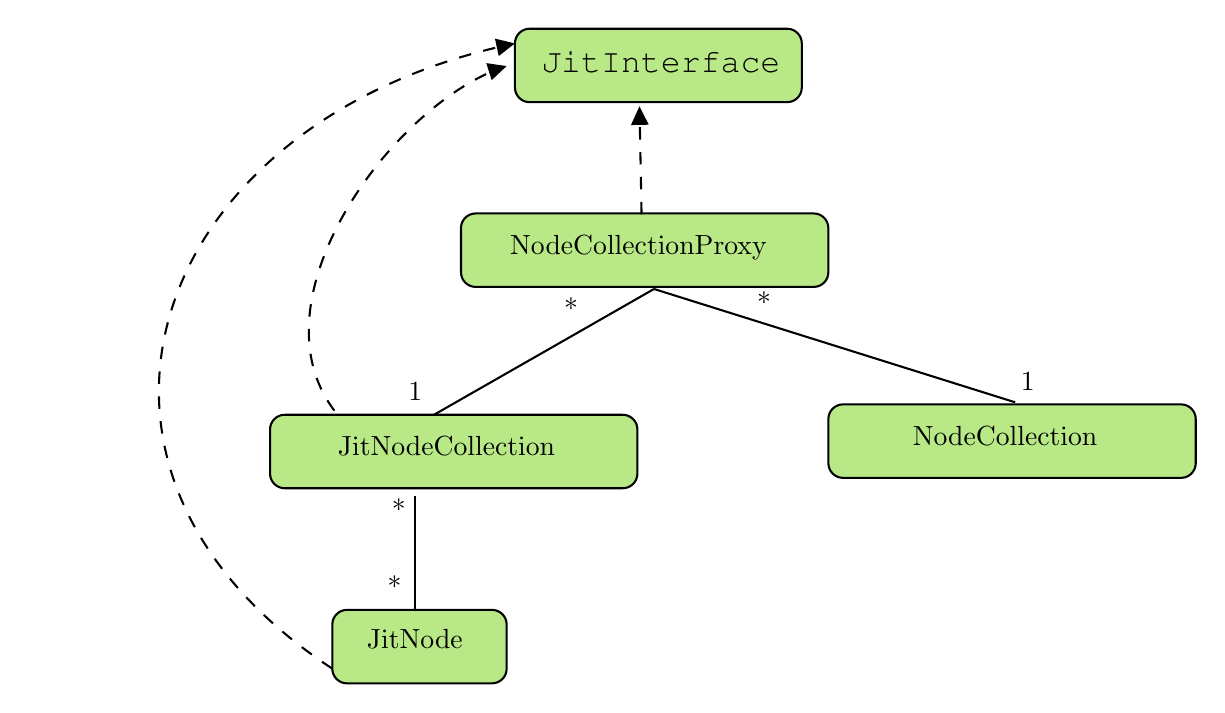
\begin{tikzpicture}[x=0.75pt,y=0.75pt,yscale=-1,xscale=1]
%uncomment if require: \path (0,539); %set diagram left start at 0, and has height of 539

%Rounded Rect [id:dp9242718804018157]
\draw  [fill={rgb, 255:red, 184; green, 233; blue, 134 }  ,fill opacity=1 ] (258.8,21.08) .. controls (258.8,17.17) and (261.97,14) .. (265.88,14) -- (389.92,14) .. controls (393.83,14) and (397,17.17) .. (397,21.08) -- (397,42.32) .. controls (397,46.23) and (393.83,49.4) .. (389.92,49.4) -- (265.88,49.4) .. controls (261.97,49.4) and (258.8,46.23) .. (258.8,42.32) -- cycle ;
%Rounded Rect [id:dp20300555302885148]
\draw  [fill={rgb, 255:red, 184; green, 233; blue, 134 }  ,fill opacity=1 ] (232.8,110.08) .. controls (232.8,106.17) and (235.97,103) .. (239.88,103) -- (402.72,103) .. controls (406.63,103) and (409.8,106.17) .. (409.8,110.08) -- (409.8,131.32) .. controls (409.8,135.23) and (406.63,138.4) .. (402.72,138.4) -- (239.88,138.4) .. controls (235.97,138.4) and (232.8,135.23) .. (232.8,131.32) -- cycle ;
%Rounded Rect [id:dp30259215827088815]
\draw  [fill={rgb, 255:red, 184; green, 233; blue, 134 }  ,fill opacity=1 ] (140.8,207.08) .. controls (140.8,203.17) and (143.97,200) .. (147.88,200) -- (310.72,200) .. controls (314.63,200) and (317.8,203.17) .. (317.8,207.08) -- (317.8,228.32) .. controls (317.8,232.23) and (314.63,235.4) .. (310.72,235.4) -- (147.88,235.4) .. controls (143.97,235.4) and (140.8,232.23) .. (140.8,228.32) -- cycle ;
%Rounded Rect [id:dp43198649276984225]
\draw  [fill={rgb, 255:red, 184; green, 233; blue, 134 }  ,fill opacity=1 ] (409.8,202.08) .. controls (409.8,198.17) and (412.97,195) .. (416.88,195) -- (579.72,195) .. controls (583.63,195) and (586.8,198.17) .. (586.8,202.08) -- (586.8,223.32) .. controls (586.8,227.23) and (583.63,230.4) .. (579.72,230.4) -- (416.88,230.4) .. controls (412.97,230.4) and (409.8,227.23) .. (409.8,223.32) -- cycle ;
%Rounded Rect [id:dp48495283974854675]
\draw  [fill={rgb, 255:red, 184; green, 233; blue, 134 }  ,fill opacity=1 ] (170.8,301.08) .. controls (170.8,297.17) and (173.97,294) .. (177.88,294) -- (247.72,294) .. controls (251.63,294) and (254.8,297.17) .. (254.8,301.08) -- (254.8,322.32) .. controls (254.8,326.23) and (251.63,329.4) .. (247.72,329.4) -- (177.88,329.4) .. controls (173.97,329.4) and (170.8,326.23) .. (170.8,322.32) -- cycle ;
%Straight Lines [id:da6129642388796104]
\draw  [dash pattern={on 4.5pt off 4.5pt}]  (319.8,103.4) -- (318.86,54.4) ;
\draw [shift={(318.8,51.4)}, rotate = 88.9] [fill={rgb, 255:red, 0; green, 0; blue, 0 }  ][line width=0.08]  [draw opacity=0] (8.93,-4.29) -- (0,0) -- (8.93,4.29) -- cycle    ;
%Straight Lines [id:da6467267156877796]
\draw    (325.8,139.4) -- (219.8,200) ;
%Straight Lines [id:da8772895818783546]
\draw    (325.8,139.4) -- (499.8,194) ;
%Straight Lines [id:da30029502415377296]
\draw    (210.8,239) -- (210.8,294) ;
%Curve Lines [id:da8958556393051575]
\draw  [dash pattern={on 4.5pt off 4.5pt}]  (171.8,198) .. controls (131.41,144.81) and (198.72,51.84) .. (252.36,32.82) ;
\draw [shift={(254.8,32)}, rotate = 162.53] [fill={rgb, 255:red, 0; green, 0; blue, 0 }  ][line width=0.08]  [draw opacity=0] (8.93,-4.29) -- (0,0) -- (8.93,4.29) -- cycle    ;
%Curve Lines [id:da7566913699794227]
\draw  [dash pattern={on 4.5pt off 4.5pt}]  (170.8,322.32) .. controls (24.53,226.48) and (81.23,59.68) .. (256.15,21.64) ;
\draw [shift={(258.8,21.08)}, rotate = 167.73] [fill={rgb, 255:red, 0; green, 0; blue, 0 }  ][line width=0.08]  [draw opacity=0] (8.93,-4.29) -- (0,0) -- (8.93,4.29) -- cycle    ;

% Text Node
\draw (270,23) node [anchor=north west][inner sep=0.75pt]   [align=left] {{\fontfamily{pcr}\selectfont {\large JitInterface}}};
% Text Node
\draw (255,112) node [anchor=north west][inner sep=0.75pt]   [align=left] {NodeCollectionProxy};
% Text Node
\draw (172,209) node [anchor=north west][inner sep=0.75pt]   [align=left] {JitNodeCollection};
% Text Node
\draw (449,204) node [anchor=north west][inner sep=0.75pt]   [align=left] {NodeCollection};
% Text Node
\draw (186,302) node [anchor=north west][inner sep=0.75pt]   [align=left] {JitNode};
% Text Node
\draw (206,183) node [anchor=north west][inner sep=0.75pt]   [align=left] {1};
% Text Node
\draw (501,178) node [anchor=north west][inner sep=0.75pt]   [align=left] {1};
% Text Node
\draw (374,139) node [anchor=north west][inner sep=0.75pt]   [align=left] {*};
% Text Node
\draw (281,142) node [anchor=north west][inner sep=0.75pt]   [align=left] {*};
% Text Node
\draw (196,276) node [anchor=north west][inner sep=0.75pt]   [align=left] {*};
% Text Node
\draw (198,239) node [anchor=north west][inner sep=0.75pt]   [align=left] {*};


\end{tikzpicture}
}
    \caption{The NodeCollectionProxy design: The \texttt{NodeCollectionProxy} can be considered a \emph{tree-like} structure with at most two children. The first (left) child is the \texttt{JitNodeCollection}, the second (right) child is the \texttt{nest.NodeCollection} class. The \texttt{JitNodeCollection} has a \emph{sub-tree} attached to it and may have an arbitrary number of children. The children of the \texttt{JitNodeCollection} are instances of the \texttt{JitNode}. The \texttt{JitInterface} provides common functionalities for retrieving the value of an item, updating it or indexing and slicing the collection. The interface is implemented by the \texttt{NodeCollection}, \texttt{JitNodeCollection} and the \texttt{JitNode}.}
    \label{fig:node_collection_proxy}
\end{figure}

\autoref{fig:node_collection_proxy} shows the essential elements for making the JIT mechanism work in the background without enforcing any changes in the simulation script or the way how the user uses the PyNEST module. We will explain the items in the figure from the bottom to the top. The \texttt{JitNode} always represents a contiguous space of the model's instances. It stores only the first and last ID of that contiguous space, and it is the only class that can directly modify the created instances, such that any query or modification to the single instances are processed at the \texttt{JitNode} level. Next we have the \texttt{JitNodeCollection}, which a collection of \texttt{JitNode}s. The \texttt{JitNodeCollection} is similar to the \texttt{NodeCollection} and provides the same functionalities. As the \texttt{JitNodeCollection} holds a list of \texttt{JitNode}s, which themselves point to a contiguous space, \emph{slicing} and \emph{indexing} of these classes is a bit more complicated and slightly different from the \texttt{NodeCollection}. Finally, we have the \texttt{NodeCollectionProxy} that has at most two \emph{children}, the \texttt{NodeCollection} and the \texttt{JitNodeCollection}. The class provides the same logic as the \texttt{NodeCollection}, but at the same time allows using the \emph{lightweight} instances after calls to the \texttt{Create()} function.

Since the relation between the classes is \emph{tree-like}, they all share the same logic for \emph{indexing}, \emph{slicing} and retrieving or modifying certain elements. To ease this, the classes implement the same \emph{interface}, preventing us from duplicating the implementation of the afforementioned functionalities.

\begin{figure}[ht!]
\centering
\begin{lstlisting}[language=Python, label=lst:jit_interface, caption={The JitInterface}]
class JitInterface():
    def get_children(self):
        pass
    def get_number_of_children(self):
        pass
    def get_keys(self):
        pass
    def get_relative_pos(self, global_pos):
        pass
    def __iter__(self):
        pass
    def project_dict(self, dict):
        pass
    def get_tuples(self, items):
        pass
    def get(self, *args. **kwargs):
        pass
    def set(self, params=None, **kwargs):
        pass
    def get_node_at(self, global_pos):
        pass
    def __getitem__(self, key):
        pass
\end{lstlisting}
%\caption{The \texttt{JitInterface}}
%\label{fig:jit_interface}
\end{figure}

The \texttt{NodeCollection} is simply a list of IDs pointing to the real instances of the model in the \texttt{NestKernel}. Mapping the list structure to a \emph{tree-like} structure requires certain functionalities in the \texttt{JitInterface} that allow a smooth conversion. The \texttt{get\_children()} function returns the direct successors. In the case of the \texttt{NodeCollectionProxy}, the direct successors are the \texttt{JitNodeCollection} and the \texttt{NodeCollection}. For the \texttt{JitNodeCollection}, the successors are instances of the \texttt{JitNode}s. The \texttt{get\_number\_of\_children()} function returns the number of successors, for the \texttt{NodeCollectionProxy} that would be at most two, and it is important to note here that this is different from adding the size of the \texttt{JitNodeCollection} with the size of the \texttt{NodeCollection}. The \texttt{get\_keys()} function returns a list of strings containing the model attributes names. The \texttt{get\_relative\_pos()} function converts a global position to a local position in the node. The range of the global IDs in the \texttt{NodeCollectionProxy} is in $[0, \texttt{len(NodeCollection)} + \texttt{len(JitNodeCollection)})$, while it is is in $[0,\sum_{n \in \texttt{JitNodes}} \texttt{len(n)}]$ in the \texttt{JitNodeCollection}. The \texttt{\_\_iter\_\_()} function is for making each of the classes \emph{iterable}. The \texttt{project\_dict} is for splitting the dictionary object into sub-dictionaries containing the new values to be set for each instance of the model. All other functions are \emph{helper} functions that support the work of the above-mentioned functions.

  
\begin{figure}[ht!]
    \centering
\tikzset{every picture/.style={line width=0.75pt}} %set default line width to 0.75pt
\scalebox{0.5}{
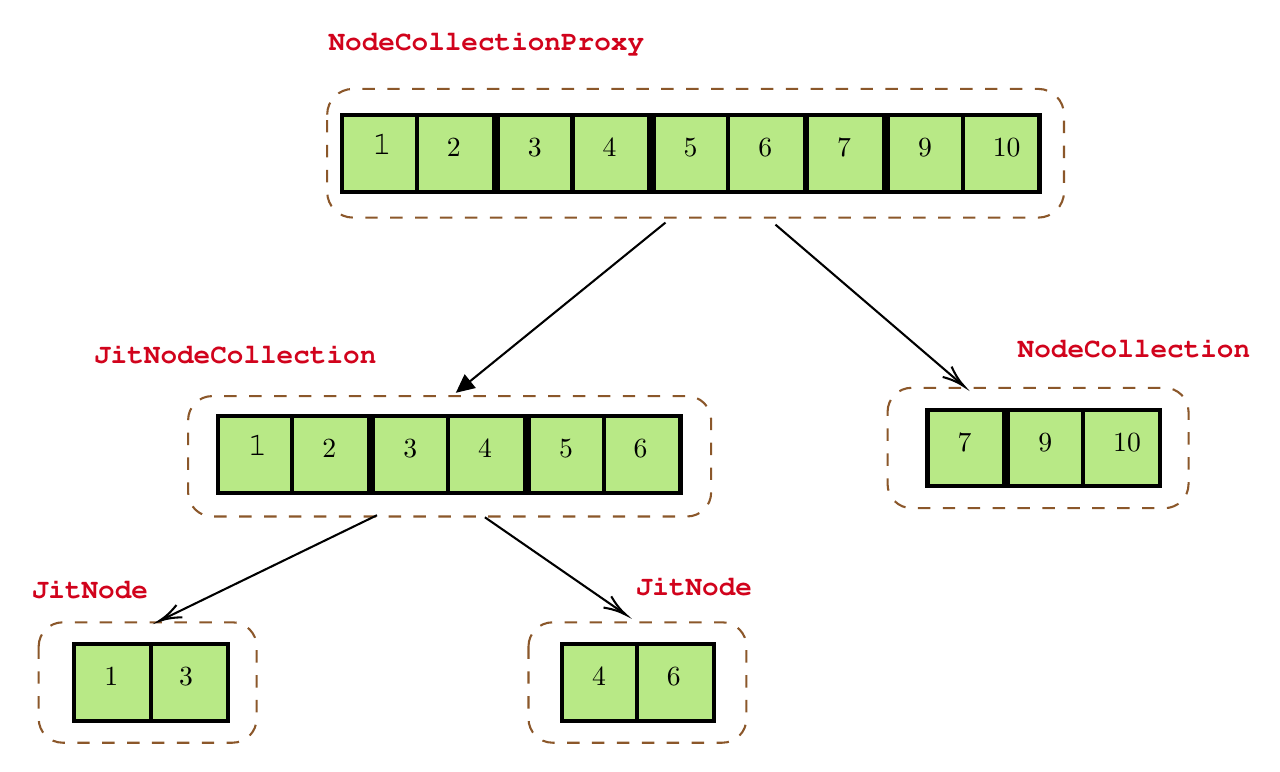
\begin{tikzpicture}[x=0.75pt,y=0.75pt,yscale=-1,xscale=1]
%uncomment if require: \path (0,426); %set diagram left start at 0, and has height of 426

%Shape: Square [id:dp8105017417201583]
\draw  [color={rgb, 255:red, 0; green, 0; blue, 0 }  ,draw opacity=1 ][fill={rgb, 255:red, 184; green, 233; blue, 134 }  ,fill opacity=1 ][line width=1.5]  (164,92.5) -- (201,92.5) -- (201,129.5) -- (164,129.5) -- cycle ;
%Shape: Square [id:dp3649335086618113]
\draw  [color={rgb, 255:red, 0; green, 0; blue, 0 }  ,draw opacity=1 ][fill={rgb, 255:red, 184; green, 233; blue, 134 }  ,fill opacity=1 ][line width=1.5]  (200,92.5) -- (237,92.5) -- (237,129.5) -- (200,129.5) -- cycle ;
%Shape: Square [id:dp6382262654140751]
\draw  [color={rgb, 255:red, 0; green, 0; blue, 0 }  ,draw opacity=1 ][fill={rgb, 255:red, 184; green, 233; blue, 134 }  ,fill opacity=1 ][line width=1.5]  (239,92.5) -- (276,92.5) -- (276,129.5) -- (239,129.5) -- cycle ;
%Shape: Square [id:dp8010542992513336]
\draw  [color={rgb, 255:red, 0; green, 0; blue, 0 }  ,draw opacity=1 ][fill={rgb, 255:red, 184; green, 233; blue, 134 }  ,fill opacity=1 ][line width=1.5]  (275,92.5) -- (312,92.5) -- (312,129.5) -- (275,129.5) -- cycle ;
%Shape: Square [id:dp31326160350937027]
\draw  [color={rgb, 255:red, 0; green, 0; blue, 0 }  ,draw opacity=1 ][fill={rgb, 255:red, 184; green, 233; blue, 134 }  ,fill opacity=1 ][line width=1.5]  (314,92.5) -- (351,92.5) -- (351,129.5) -- (314,129.5) -- cycle ;
%Shape: Square [id:dp4264806381468127]
\draw  [color={rgb, 255:red, 0; green, 0; blue, 0 }  ,draw opacity=1 ][fill={rgb, 255:red, 184; green, 233; blue, 134 }  ,fill opacity=1 ][line width=1.5]  (350,92.5) -- (387,92.5) -- (387,129.5) -- (350,129.5) -- cycle ;
%Shape: Square [id:dp0657777285734038]
\draw  [color={rgb, 255:red, 0; green, 0; blue, 0 }  ,draw opacity=1 ][fill={rgb, 255:red, 184; green, 233; blue, 134 }  ,fill opacity=1 ][line width=1.5]  (388,92.5) -- (425,92.5) -- (425,129.5) -- (388,129.5) -- cycle ;
%Shape: Square [id:dp9110731509942587]
\draw  [color={rgb, 255:red, 0; green, 0; blue, 0 }  ,draw opacity=1 ][fill={rgb, 255:red, 184; green, 233; blue, 134 }  ,fill opacity=1 ][line width=1.5]  (427,92.5) -- (464,92.5) -- (464,129.5) -- (427,129.5) -- cycle ;
%Shape: Square [id:dp8397495965826969]
\draw  [color={rgb, 255:red, 0; green, 0; blue, 0 }  ,draw opacity=1 ][fill={rgb, 255:red, 184; green, 233; blue, 134 }  ,fill opacity=1 ][line width=1.5]  (463,92.5) -- (500,92.5) -- (500,129.5) -- (463,129.5) -- cycle ;
%Shape: Square [id:dp010231923951544264]
\draw  [color={rgb, 255:red, 0; green, 0; blue, 0 }  ,draw opacity=1 ][fill={rgb, 255:red, 184; green, 233; blue, 134 }  ,fill opacity=1 ][line width=1.5]  (104,237.5) -- (141,237.5) -- (141,274.5) -- (104,274.5) -- cycle ;
%Shape: Square [id:dp40727955432554497]
\draw  [color={rgb, 255:red, 0; green, 0; blue, 0 }  ,draw opacity=1 ][fill={rgb, 255:red, 184; green, 233; blue, 134 }  ,fill opacity=1 ][line width=1.5]  (140,237.5) -- (177,237.5) -- (177,274.5) -- (140,274.5) -- cycle ;
%Shape: Square [id:dp569596288283355]
\draw  [color={rgb, 255:red, 0; green, 0; blue, 0 }  ,draw opacity=1 ][fill={rgb, 255:red, 184; green, 233; blue, 134 }  ,fill opacity=1 ][line width=1.5]  (179,237.5) -- (216,237.5) -- (216,274.5) -- (179,274.5) -- cycle ;
%Shape: Square [id:dp7015769826403364]
\draw  [color={rgb, 255:red, 0; green, 0; blue, 0 }  ,draw opacity=1 ][fill={rgb, 255:red, 184; green, 233; blue, 134 }  ,fill opacity=1 ][line width=1.5]  (215,237.5) -- (252,237.5) -- (252,274.5) -- (215,274.5) -- cycle ;
%Shape: Square [id:dp6481677925435276]
\draw  [color={rgb, 255:red, 0; green, 0; blue, 0 }  ,draw opacity=1 ][fill={rgb, 255:red, 184; green, 233; blue, 134 }  ,fill opacity=1 ][line width=1.5]  (254,237.5) -- (291,237.5) -- (291,274.5) -- (254,274.5) -- cycle ;
%Shape: Square [id:dp5988881062447686]
\draw  [color={rgb, 255:red, 0; green, 0; blue, 0 }  ,draw opacity=1 ][fill={rgb, 255:red, 184; green, 233; blue, 134 }  ,fill opacity=1 ][line width=1.5]  (290,237.5) -- (327,237.5) -- (327,274.5) -- (290,274.5) -- cycle ;
%Shape: Square [id:dp3368376702520288]
\draw  [color={rgb, 255:red, 0; green, 0; blue, 0 }  ,draw opacity=1 ][fill={rgb, 255:red, 184; green, 233; blue, 134 }  ,fill opacity=1 ][line width=1.5]  (446,234.5) -- (483,234.5) -- (483,271.5) -- (446,271.5) -- cycle ;
%Shape: Square [id:dp8793990825777143]
\draw  [color={rgb, 255:red, 0; green, 0; blue, 0 }  ,draw opacity=1 ][fill={rgb, 255:red, 184; green, 233; blue, 134 }  ,fill opacity=1 ][line width=1.5]  (485,234.5) -- (522,234.5) -- (522,271.5) -- (485,271.5) -- cycle ;
%Shape: Square [id:dp5464263246257259]
\draw  [color={rgb, 255:red, 0; green, 0; blue, 0 }  ,draw opacity=1 ][fill={rgb, 255:red, 184; green, 233; blue, 134 }  ,fill opacity=1 ][line width=1.5]  (521,234.5) -- (558,234.5) -- (558,271.5) -- (521,271.5) -- cycle ;
%Shape: Square [id:dp7930487300244025]
\draw  [color={rgb, 255:red, 0; green, 0; blue, 0 }  ,draw opacity=1 ][fill={rgb, 255:red, 184; green, 233; blue, 134 }  ,fill opacity=1 ][line width=1.5]  (35,347.5) -- (72,347.5) -- (72,384.5) -- (35,384.5) -- cycle ;
%Shape: Square [id:dp5303377541943575]
\draw  [color={rgb, 255:red, 0; green, 0; blue, 0 }  ,draw opacity=1 ][fill={rgb, 255:red, 184; green, 233; blue, 134 }  ,fill opacity=1 ][line width=1.5]  (72,347.5) -- (109,347.5) -- (109,384.5) -- (72,384.5) -- cycle ;
%Shape: Square [id:dp8774571362079038]
\draw  [color={rgb, 255:red, 0; green, 0; blue, 0 }  ,draw opacity=1 ][fill={rgb, 255:red, 184; green, 233; blue, 134 }  ,fill opacity=1 ][line width=1.5]  (270,347.5) -- (307,347.5) -- (307,384.5) -- (270,384.5) -- cycle ;
%Shape: Square [id:dp5060305166010015]
\draw  [color={rgb, 255:red, 0; green, 0; blue, 0 }  ,draw opacity=1 ][fill={rgb, 255:red, 184; green, 233; blue, 134 }  ,fill opacity=1 ][line width=1.5]  (306,347.5) -- (343,347.5) -- (343,384.5) -- (306,384.5) -- cycle ;
%Rounded Rect [id:dp7324795238782251]
\draw  [color={rgb, 255:red, 139; green, 87; blue, 42 }  ,draw opacity=1 ][dash pattern={on 4.5pt off 4.5pt}] (156.8,92.4) .. controls (156.8,85.55) and (162.35,80) .. (169.2,80) -- (499.4,80) .. controls (506.25,80) and (511.8,85.55) .. (511.8,92.4) -- (511.8,129.6) .. controls (511.8,136.45) and (506.25,142) .. (499.4,142) -- (169.2,142) .. controls (162.35,142) and (156.8,136.45) .. (156.8,129.6) -- cycle ;
%Rounded Rect [id:dp8536055044343349]
\draw  [color={rgb, 255:red, 139; green, 87; blue, 42 }  ,draw opacity=1 ][dash pattern={on 4.5pt off 4.5pt}] (89.8,239.6) .. controls (89.8,233.19) and (94.99,228) .. (101.4,228) -- (330.2,228) .. controls (336.61,228) and (341.8,233.19) .. (341.8,239.6) -- (341.8,274.4) .. controls (341.8,280.81) and (336.61,286) .. (330.2,286) -- (101.4,286) .. controls (94.99,286) and (89.8,280.81) .. (89.8,274.4) -- cycle ;
%Rounded Rect [id:dp7918544993903414]
\draw  [color={rgb, 255:red, 139; green, 87; blue, 42 }  ,draw opacity=1 ][dash pattern={on 4.5pt off 4.5pt}] (426.8,235.6) .. controls (426.8,229.19) and (431.99,224) .. (438.4,224) -- (560.2,224) .. controls (566.61,224) and (571.8,229.19) .. (571.8,235.6) -- (571.8,270.4) .. controls (571.8,276.81) and (566.61,282) .. (560.2,282) -- (438.4,282) .. controls (431.99,282) and (426.8,276.81) .. (426.8,270.4) -- cycle ;
%Rounded Rect [id:dp667353387028452]
\draw  [color={rgb, 255:red, 139; green, 87; blue, 42 }  ,draw opacity=1 ][dash pattern={on 4.5pt off 4.5pt}] (253.8,348.6) .. controls (253.8,342.19) and (258.99,337) .. (265.4,337) -- (347.2,337) .. controls (353.61,337) and (358.8,342.19) .. (358.8,348.6) -- (358.8,383.4) .. controls (358.8,389.81) and (353.61,395) .. (347.2,395) -- (265.4,395) .. controls (258.99,395) and (253.8,389.81) .. (253.8,383.4) -- cycle ;
%Rounded Rect [id:dp8903611832797551]
\draw  [color={rgb, 255:red, 139; green, 87; blue, 42 }  ,draw opacity=1 ][dash pattern={on 4.5pt off 4.5pt}] (17.8,348.6) .. controls (17.8,342.19) and (22.99,337) .. (29.4,337) -- (111.2,337) .. controls (117.61,337) and (122.8,342.19) .. (122.8,348.6) -- (122.8,383.4) .. controls (122.8,389.81) and (117.61,395) .. (111.2,395) -- (29.4,395) .. controls (22.99,395) and (17.8,389.81) .. (17.8,383.4) -- cycle ;
%Straight Lines [id:da10260503749552963]
\draw    (319.8,144.4) -- (221.13,224.51) ;
\draw [shift={(218.8,226.4)}, rotate = 320.93] [fill={rgb, 255:red, 0; green, 0; blue, 0 }  ][line width=0.08]  [draw opacity=0] (8.93,-4.29) -- (0,0) -- (8.93,4.29) -- cycle    ;
%Straight Lines [id:da9877013332650502]
\draw    (372.8,145.4) -- (462.28,222.1) ;
\draw [shift={(463.8,223.4)}, rotate = 220.6] [color={rgb, 255:red, 0; green, 0; blue, 0 }  ][line width=0.75]    (10.93,-3.29) .. controls (6.95,-1.4) and (3.31,-0.3) .. (0,0) .. controls (3.31,0.3) and (6.95,1.4) .. (10.93,3.29)   ;
%Straight Lines [id:da062130966082328376]
\draw    (180.8,285.4) -- (77.6,335.53) ;
\draw [shift={(75.8,336.4)}, rotate = 334.09] [color={rgb, 255:red, 0; green, 0; blue, 0 }  ][line width=0.75]    (10.93,-3.29) .. controls (6.95,-1.4) and (3.31,-0.3) .. (0,0) .. controls (3.31,0.3) and (6.95,1.4) .. (10.93,3.29)   ;
%Straight Lines [id:da44240203700368275]
\draw    (232.8,286.4) -- (299.15,332.26) ;
\draw [shift={(300.8,333.4)}, rotate = 214.65] [color={rgb, 255:red, 0; green, 0; blue, 0 }  ][line width=0.75]    (10.93,-3.29) .. controls (6.95,-1.4) and (3.31,-0.3) .. (0,0) .. controls (3.31,0.3) and (6.95,1.4) .. (10.93,3.29)   ;

% Text Node
\draw (177,100.5) node [anchor=north west][inner sep=0.75pt]   [align=left] {{\fontfamily{pcr}\selectfont {\large 1}}};
% Text Node
\draw (213,102.5) node [anchor=north west][inner sep=0.75pt]   [align=left] {2};
% Text Node
\draw (252,102.5) node [anchor=north west][inner sep=0.75pt]   [align=left] {3};
% Text Node
\draw (288,102.5) node [anchor=north west][inner sep=0.75pt]   [align=left] {4};
% Text Node
\draw (327,102.5) node [anchor=north west][inner sep=0.75pt]   [align=left] {5};
% Text Node
\draw (363,102.5) node [anchor=north west][inner sep=0.75pt]   [align=left] {6};
% Text Node
\draw (401,102.5) node [anchor=north west][inner sep=0.75pt]   [align=left] {7};
% Text Node
\draw (440,102.5) node [anchor=north west][inner sep=0.75pt]   [align=left] {9};
% Text Node
\draw (476,102.5) node [anchor=north west][inner sep=0.75pt]   [align=left] {10};
% Text Node
\draw (117,245.5) node [anchor=north west][inner sep=0.75pt]   [align=left] {{\fontfamily{pcr}\selectfont {\large 1}}};
% Text Node
\draw (153,247.5) node [anchor=north west][inner sep=0.75pt]   [align=left] {2};
% Text Node
\draw (192,247.5) node [anchor=north west][inner sep=0.75pt]   [align=left] {3};
% Text Node
\draw (228,247.5) node [anchor=north west][inner sep=0.75pt]   [align=left] {4};
% Text Node
\draw (267,247.5) node [anchor=north west][inner sep=0.75pt]   [align=left] {5};
% Text Node
\draw (303,247.5) node [anchor=north west][inner sep=0.75pt]   [align=left] {6};
% Text Node
\draw (459,244.5) node [anchor=north west][inner sep=0.75pt]   [align=left] {7};
% Text Node
\draw (498,244.5) node [anchor=north west][inner sep=0.75pt]   [align=left] {9};
% Text Node
\draw (534,244.5) node [anchor=north west][inner sep=0.75pt]   [align=left] {10};
% Text Node
\draw (48,357.5) node [anchor=north west][inner sep=0.75pt]   [align=left] {1};
% Text Node
\draw (84,357.5) node [anchor=north west][inner sep=0.75pt]   [align=left] {3};
% Text Node
\draw (283,357.5) node [anchor=north west][inner sep=0.75pt]   [align=left] {4};
% Text Node
\draw (319,357.5) node [anchor=north west][inner sep=0.75pt]   [align=left] {6};
% Text Node
\draw (43,202) node [anchor=north west][inner sep=0.75pt]   [align=left] {{\fontfamily{pcr}\selectfont \textcolor[rgb]{0.82,0.01,0.11}{\textbf{JitNodeCollection}}}};
% Text Node
\draw (488,199) node [anchor=north west][inner sep=0.75pt]   [align=left] {{\fontfamily{pcr}\selectfont \textcolor[rgb]{0.82,0.01,0.11}{\textbf{NodeCollection}}}};
% Text Node
\draw (13,315) node [anchor=north west][inner sep=0.75pt]   [align=left] {{\fontfamily{pcr}\selectfont \textcolor[rgb]{0.82,0.01,0.11}{\textbf{JitNode}}}};
% Text Node
\draw (304,314) node [anchor=north west][inner sep=0.75pt]   [align=left] {{\fontfamily{pcr}\selectfont \textcolor[rgb]{0.82,0.01,0.11}{\textbf{JitNode}}}};
% Text Node
\draw (156,51) node [anchor=north west][inner sep=0.75pt]   [align=left] {{\fontfamily{pcr}\selectfont \textcolor[rgb]{0.82,0.01,0.11}{\textbf{NodeCollectionProxy}}}};

\end{tikzpicture}
}
    \caption{From list to \emph{tree-like} structure: The initial \texttt{NodeCollectionProxy} has 9 items. The first 6 items are from the \texttt{JitNodeCollection} and the last 3 are from the \texttt{nest.NodeCollection}. The six items  in \texttt{JitNodeCollection} are from two different models, and these instances of the models are represented by the \texttt{JitNode}. The first \texttt{JitNode} spans a contiguous space of \emph{ids} between 1 and 3. The second \texttt{JitNode} spans another contiguous space between 4 and 6.}
    \label{fig:list_to_tree}
\end{figure}

Due to the \emph{tree-like} structure of the \texttt{NodeCollectionProxy} (depicted in \autoref{fig:list_to_tree}), retrieving an element from the \texttt{NodeCollection} at position $i$ is not a very straightforward task. Since the root only has two child nodes, we can first check if $i$ is less than the size of the \texttt{JitNodeCollection}, otherwise we continue our search in the \texttt{NodeCollection}. If $i$ ends up being in the range of the \texttt{JitNodeCollection}, we check if $i$ belongs to one of the \texttt{JitNode} blocks. Assuming we have $n$ \texttt{JitNode} blocks and each block points to $k_j$ instances of any arbitrary model $m$ for $j \in [1, n]$, a \texttt{JitNode} block $b_l$ is selected with $l \in [1, n)$ if $\sum_{j=1}^{l-1} \text{len}(b_j) \leq i < \sum_{j=1}^{l-1} \text{len}(b_j) + \text{len}(b_l)$. Once the block $b$ is found, we can convert the global ID $i$ to a \emph{local} id with respect to the found block $b_l$. Thus, the local ID is computed as $\text{id}_\text{local} = i -\sum_{j=1}^{l-1} \text{len}(b_j)$. Since the \texttt{JitNode} is \emph{indexable}, we can simply get a new \texttt{JitNode} having the \texttt{first} attribute set to the local ID and the \texttt{last} attribute to the value $\text{id}_\text{local} + 1$, and the \texttt{model\_name} to $m$.

The result for querying the \texttt{NodeCollectionProxy} for the element at position $i$ will then be a new \texttt{NodeCollectionProxy} with a size of one, and it contains only a \texttt{JitNodeCollection}. The \texttt{JitNodeCollection} instance will have a single \texttt{JitNode} object pointing to one element. To illustrate the algorithm using an example, let's take the \texttt{NodeCollectionProxy} in \autoref{fig:list_to_tree} with ten elements and let $i = 5$. The \texttt{JitNodeCollection} has six elements and the \texttt{NodeCollection} has only four, therefore $i=5$ ends up in the \texttt{JitNodeCollection} child. For the first \texttt{JitNode} in the \texttt{JitNodeCollection} we have three items, in the second one we have two elements, and therefore we have $l \in \{1, 2\}$. For $l = 1$, we have $0 \leq i = 5$ and $5 \not < 0 + \text{len}(b_l) = 0 + \text{len}(b_1) = 0 + 3 = 3$. For $l = 2$, we have $0 + \text{len}(b_1) = 0 + 3 \leq 5$ and $5 < \text{len}(b_1) + \text{len}(b_2) = 3 + 3 = 6$. In this case, it seems that $l = 2$ satisfies the required condition, and therefore $i = 5$ belongs to the second \texttt{JitNode} block. The result then will be a \texttt{NodeCollectionProxy} with only a \texttt{JitNodeCollection} child, which has a single \texttt{JitNode} with attributes \texttt{first=5-4}, \texttt{last=6}, \texttt{name=$m$>}, with 4 being the index where the second \texttt{JitNode} starts and $m$ the name of the model.

\emph{Slicing} a \texttt{NodeCollectionProxy} is similar to indexing, with the only difference that we have a sequence of items $(a_1, \dots, a_k)$, with $k$ the size of the sequence. The problem with \emph{slicing} is that the items are not necessary the direct successors of each other. In other words, it may be that $a_{i+1} =a_i + l$, for $l > 1$, and $a_i$ and $a_{i+1}$ might point to different \texttt{JitNode}s. In order to solve this problem, we start by mapping each $a_i$ to the corresponding \texttt{JitNode} block, then we group all items together that share the same block. For each group, we convert the global IDs $a_i$ to the relative local IDs in each \texttt{JitNode} block. By doing so, we get the following mapping: $(a_1, a_2, \dots, a_k) \mapsto (P_1, \dots P_l)$, with $\lvert\bigcup_{i=1}^{l} P_{i}\rvert =n$. $P_i$ is the partition of the items containing the local IDs of the original sequence. For each partition $P_i$, we aggregate the elements inside them in a way that each group is a contiguous group of IDs. Each of these groups then constructs a new \texttt{JitNode} and all the new \texttt{JitNode}s will be packed in a new \texttt{JitNodeCollection}.

Basically, for \emph{indexing} and \emph{slicing}, we iterate over the \emph{tree-like} structure twice. In the first iteration, we examine the tree from the top to the bottom by mapping the global IDs to local IDs and retrieve the correct \texttt{JitNode} instances. In the second iteration, we traverse the tree from the bottom to the top by merging and aggregating the results together until constructing the final \texttt{NodeCollectionProxy}. Getting or setting the value of certain \emph{keys} in the \texttt{NodeCollectionProxy} follows the same logic. By requesting the value of some \emph{keys}, the \texttt{NodeCollectionProxy} asks both the \texttt{NodeCollection} and the \texttt{JitNodeCollection} to retrieve the value for the given keys. In return, the \texttt{JitNodeCollection} does the same by asking each of the \texttt{JitNode} blocks. The returned value will be either the correct value that is stored in instances of the model or a \texttt{NoneType} object, indicating that the model does not have the requested \emph{key} as an attribute. Again, the result from each level will be aggregated and delivered to a higher level in the tree until we reach the root (i.e., the \texttt{NodeCollectionProxy}). The \texttt{set()} function in the \texttt{NodeCollectionProxy} has the exact same behavior as the \texttt{get()} function, with the only difference that the new values will be split among the children in a way that each child gets a sub-dictionary containing only its own \emph{keys}.

\subsection{The \texttt{JitModelParser}}

Generating the code for the \emph{lightweight} version of the model basically follows the same logic as generating the code for the whole library. The \texttt{JitModelParser} is the component responsible for creating the \emph{lightweight} version. It takes the \texttt{ASTNeuron} as an input and returns \texttt{C++} code as an output. The \texttt{C++} code contains the \emph{State} and the \emph{Parameter} blocks, including the \emph{constructor} that initializes the block's attributes. As some of these attributes might be assigned a random value drawn from a distribution in the NestKernel, we run into the problem that the random number generator belongs to the \texttt{NestKernel}, to which we do not have access at this point in the processing pipeline. Furthermore, it is very important to preserve the order in which the random numbers are drawn to ensure the perfect \emph{reproducibility} of the simulation results.

To tackle this problem, the \texttt{JitModelParser} extracts the \emph{symbols} referring to the random number generator in the generated \texttt{C++} code for the \emph{lightweight} version from the constructor and replaces them with a variable, whose declaration will be inserted back into the constructor. If we now have $n$ statements in the constructor that use a random number generator in their expression, we replace the occurrences of each of these generators with a new variable $r_i$, for $i \in [1, n]$ and extend the constructor with $n$ new parameters in the form of $\texttt{double} r_i$. The \texttt{JitModelParse} compiles the \emph{lightweight} version and makes the new class available in the Python interface with the help of the \emph{CPPYY} module \citep{cppyy}. The \texttt{JitModelParser} is then also responsible for calling the extended constructor, and provides the value of the newly added parameters by simply calling the PyNEST functions responsible for generating the random numbers and passing them to the \emph{lightweight} version class constructor to initialize its attributes in the \emph{state} and \emph{parameters} blocks.

Unfortunately, the \texttt{lightweight} version of the model leads to a duplication of the space for the attributes as we have to store them once in the \texttt{lightweight} model and a second time once we are done building the library and creating the real instance of the model. Also, as the random numbers are drawn by a single compute node, the exact numbers drawn and the performance of drawing them might differ if more compute nodes are used. To tackle this problem and partially solve it, we have come up with a new internal design to make the models more modular and decompose them into independent interchangeable subcomponents. These concepts for extended \emph{modularity} will be explained in more detail in \autoref{chap:vec}.

\section{Wrapping PyNEST: the \texttt{Connect()} function}

Previously, all neuron-synapse combinations involving synapse models with a dependency on post-synaptic variables, such as in the case of spike-timing dependent plasticity (STDP), had to be provided manually to the code generator before running the simulation. This dependency is now hidden in the \texttt{ConnectWrapper} class that extends the functionality of PyNEST's \texttt{Connect()} function. Depending on the synaptic connection, the code generation process might be triggered for the second time after being called for calls to \texttt{Create()}, but this time with different configurations that allow the co-generation of neuron model code together with its synaptic elements.

\subsection{The \texttt{ConnectWrapper}}

The \texttt{ConnectWrapper} with its three core functions (i.e., \texttt{before()}/\texttt{main()}/\texttt{after()}) intercepts the calls to the \texttt{Connect()} function in PyNEST, ensuring the correct use of models during the construction of the network. The \texttt{before()} functions has the same signature as \texttt{Connect()} itself. It takes the source and target populations and additionally two dictionaries, one for specifying the connection rule and its properties and one for specifying the synapse model and its properties. The task of the \texttt{before()} function in the context of the connection setup is to make sure that the sources and targets are available as the real instances of the models (instead of just as lightweight versions) and that the \texttt{NodeCollectionProxy} only contains a \texttt{NodeCollection} and the \texttt{JitNodeCollection} is empty.

The \texttt{before()} function starts by checking if either the target is a \texttt{NodeCollectionProxy} containing a \texttt{JitNodeCollection} child or the synapse model type is an external model. If both requirements are satisfied and, depending on the situation, if both the postsynaptic neuron model types and the synapse type are already existing in a library or coming from a \texttt{.nestml} file, the \texttt{before()} function delegates the work to the \texttt{ConnectHelper} that takes care of converting the postsynaptic nodes residing in the \texttt{JitNodeCollection} to the real instances. Next, we check if the source and target are contained inside a \texttt{JitNodeCollection}, which means there are at least two \emph{threads} running and building the code for the source and target neurons models. We then explicitly wait for these two threads, and when they finish without failure, we install the two libraries built by the threads and convert the \texttt{JitNodeCollection} objects from the source and target to the \texttt{NodeCollection} objects. Depending on the order of calling the \texttt{Connect()} function, we might need to delete certain connections and replace them with others.

From the perspective of the JIT mechanism, we do not really know what will happen to the model and which connections it will have when calling \texttt{Create()}. This will only become known when calling the \texttt{Connect()} function. If that is called using an external synapse model we will have to delete connections and replace them with others because the target neuron model will be assigned a new name by the code generation pipeline and the original target model will not be valid anymore. As the final step, the \texttt{before()} function converts the \texttt{JitNodeCollection} to a \texttt{NodeCollection} and returns it together with the other parameters as input parameters to the \texttt{main()} function in the \texttt{ConnectWrapper}. Both the \texttt{main()} and \texttt{after()} functions are the default implementation from the base class, which means that \texttt{main()} just calls the real \texttt{Connect()} function and \texttt{after()} does nothing.

\subsection{The \texttt{ConnectHelper}}

The \texttt{ConnectHelper} is responsible for checking the state of the threads that are involved in building the library of the models specified in the call to \texttt{Connect()}. It installs the libraries and converts the \texttt{JitNodeCollection} to the \texttt{NodeCollection}. It handles the use case when the co-generation pipeline must be triggered again and takes care of deleting and replacing the connections of the involved models.

The \texttt{wait\_for\_threads()} method takes a list of \emph{strings} containing the name of threads that we must wait for as argument. The thread names correspond to the names of the model they are building the library for. The function waits for the specified threads and inspects their states once they are done building the library and, depending on the state, either continues the execution of the \texttt{ConnectWrapper} or throws a failure message and stops the execution of the simulation script. Finally, the function removes the terminated threads from the list of running threads. The list will be either further processed by another call to \texttt{Connect()} or by the \texttt{Simulate()} function.

The \texttt{install\_modules()} method takes the same parameters as the  \texttt{wait\_for\_threads()} function and is responsible for installing the libraries, calling the \texttt{SetDefaults()} for models that have their default values changed, coping models by calling \texttt{CopyModels()} in case if one of the given models has different initial values.

One of the most important functions in the \texttt{ConnecetHelper} class is \texttt{convert\_post\_neuron()}, which handles the conversion of the postsynapse neuron when an external synapse model is involved. This function takes a \texttt{NodeCollectionProxy} and the name of the synapse model as parameters. Depending on the elements involved, we distinguish nine distinct cases when applying the conversion. Each of the neuron and synapse model can be either from a \texttt{.nestml} file, an \emph{external library} or an already built-in model. We can thus build a pair where the first entry indicates the source of the neuron and the second is for the source of the synapse model. The first pair is \emph{(nestml, nestml}), which means that both models are found in the NESTML format. In this case, we have the \emph{handle\_nestml\_nestml()} function that starts the code generation for the new model that exclusively supports the given synapse model. The function does not parse both models, but it retrieves them from the \texttt{JitModels} class as that has already parsed and validated them. The function only triggers the transformation phase, as some attributes from the synapse may have to be transferred to the neuron model. Once the code generation is completed and the library is installed, the function creates the real instance of the model and returns the new \texttt{NodeCollection} objects to be used further in the \texttt{main()} function in the \texttt{ConnectWrapper}.

The second pair to be considered is \emph{(external, nestml}), which occurs when the neuron model already exists in some external library and the synapse model is only available in NESTML format. In this case the function tries to find the \texttt{.nestml} version of the model, and if it is found, it will execute the same logic as in the previous case. If the \texttt{.nestml} file for the model is not found, we just throw an error and stop the execution, as it is not possible to bind the synapse with the model without having extra information how to generate the code of the \emph{neuron-synapse} model pair.

The next pair is \emph{(built-in, nestml)} case, where the neuron model is a built-in model and the synapse comes from a \texttt{.nestml} file. This case requires a prior condition to be satisfied in order to continue the execution of the \texttt{Connect()} function: In general, if the target model name is \emph{x} and the synapse name is \emph{y}, and we want to connect the source and target with using synapse \emph{y}, then the name of the target model must be \emph{x\_\_with\_y} and the synapse will be assigned a new name as \emph{y\_\_with\_x}. In general, the synapse and the neuron code are complied and built in the same library, so that if \emph{y\_\_with\_x} is installed then \emph{x\_\_with\_y} is also and vice-versa. In this particular case, we search if the synapse \emph{y\_\_with\_x} can be found in any of the existing libraries and install it, which should then also register the \emph{x\_\_with\_y} neuron model, and then we can continue creating the \texttt{NodeCollection} object.

Finally, we have \emph{(built-in, built-in)} which means that both neuron and synapse model are already available in the NestKernel. As in the previous case, it is required that both the \emph{x\_\_with\_y} and \emph{y\_\_with\_x} are registered, or we will just stop the execution of the simulation script and throw an error telling the user that we cannot find the models. In all remaining cases, we just do nothing ij the \texttt{ConnectWrapper} and let PyNEST's \texttt{Connect()} function handle them.

As the last function in the \texttt{ConnectWrapper}, we have \texttt{convert\_to\_node\_collection()} that converts an instance of the \texttt{JitNodeCollection} to a \texttt{NodeCollection} and updates the newly created instances by assigning values to the model. It is important to point out the difference between \texttt{convert\_to\_node\_collection()} and \texttt{convert\_post\_neuron()}, as the second function is only called to convert the target \texttt{NodeCollectionProxy} if there is an external synapse model involved and the first function converts any \texttt{JitNodeCollection} without any prior requirements apart from the model's library being already installed in the NestKernel.

\section{Wrapping PyNEST: The \texttt{Simulate()} function}

The \texttt{Simulate()} method of PyNEST is intercepted by the \texttt{SimulateWrapper} that works very similarly to the \texttt{ConnectWrapper}. However, instead of extracting models only from the source and target arguments as in case of the \texttt{Connect()} function, we apply the function to all models. In other words, we have to wait for all code generation threads before running PyNEST's \emph{Simulate()} function. If the code generation finishes without error, all libraries built by the threads will be installed and all \texttt{JitNodeCollection} instances existing in the simulation script will be converted to \texttt{NodeCollection} objects, including those coming from \emph{slicing} and \emph{indexing} operations. Like the other above mentioned derived \texttt{Wrapper} classes, the \texttt{SimulateWrapper} uses a helper class (\texttt{SimulateHelper}) that implements the main part of the functionalities.

\section{Usage}

\hl{While enjoyed reading the chapter up to here a lot, I find the example pretty much useless for the reader. The reason for this is that it is 1) a bit too complex for my taste (it uses a lot of modeling concepts that have not been introduced anywhere) and 2) more importantly it is impossible to see the differences between the code parts with and without JIT in the current form of the presentation as different listings. Could you either try to make the listings go side-by-side or look like the diff view for a PR on GitHub where you see deleted lines in red and added lines in green? That would make the changes much more obvious and reduce the number of different listings the reader has to scroll between.}


After the main design concepts and implementation details have been explained, we end this chapter by showing the changes that must be applied at the simulation script level to enable the JIT compilation. For the purpose of the following demonstrations, we will use the \emph{STDP windows tutorial} from the official NESTML website in order to show the adjustments required in a real-world example.

The first lines that are affected when using the JIT mechanism are directly at the beginning where modules are imported. While \autoref{lst:imports_without_jit} imports PyNEST and PyNESML and sets the path to the NEST installation, \autoref{lst:imports_with_jit} only requires a single import to make the \texttt{nest} sub-module from the JIT module available. The rest of the import lines stay unchanged.

\begin{figure}[ht!]
\centering
\begin{lstlisting}[language=Python, label=lst:imports_without_jit, caption={The Simulation script imports without JIT}]
import nest
from pynestml.frontend.pynestml_frontend import generate_nest_target
NEST_PREFIX = nest.ll_api.sli_func("statusdict/prefix ::")

%matplotlib inline
import matplotlib as mpl
mpl.rcParams['axes.formatter.useoffset'] = False
import matplotlib.pyplot as plt
import numpy as np
import os
import re
\end{lstlisting}
%\caption{The Simulation script imports without JIT}
%\label{fig:imports_without_jit}
\end{figure}

\begin{figure}[ht!]
\centering
\begin{lstlisting}[language=Python, label=lst:imports_with_jit, caption={The Simulation script imports with JIT}]
from jit import nest

%matplotlib inline
import matplotlib as mpl
mpl.rcParams['axes.formatter.useoffset'] = False
import matplotlib.pyplot as plt
import numpy as np
import os
import re
\end{lstlisting}
%\caption{The Simulation script imports JIT}
%\label{fig:imports_with_jit}
\end{figure}

Secondly, in the NESTML tutorial, we have the \texttt{generate\_code\_for} in \autoref{lst:generating_code} that takes as parameter the synapse model name. The function retrieves the \emph{nestml} file for the given synapse and also the \emph{nestml} file for the \texttt{iaf\_psc\_delta} neuron model and then triggers the co-code generation for both models together providing the \texttt{post\_ports} that required for connecting the postsynaptic neuron together with the synapse. Finally, once the code generation pipeline finishes, it installs the new library, which makes the specified model available for use in the simulation script and returns the new expected name of the neuron and synapse that both have the \emph{\_\_with\_} infix. Luckily, using JIT we can simply get rid of this huge function and let it completely take care of the models, and their new names. Even the \texttt{nest.Install} function on the line 41 will also be deleted, and only the JIT is responsible for calling it.



Finlay, we reach the part where we have to create the nodes and connect them to build the network. Both the figures \autoref{lst:build_network_with_jit} and \autoref{lst:build_network_without_jit} share the exact the code, apart from a slight difference in the line 44 when calling the \texttt{nest.Connect} function. In the figure \autoref{lst:build_network_with_jit} we add an extra key in the \texttt{syn\_spec} indicating the \emph{post connection ports} between the synapse and the post-neuron. The new key then will be removed from the \texttt{syn\_spec} dictionary and only be used in the code generation pipeline as one of the custom configurations in the \emph{codegen\_opt} in PyNESTML module. The rest of the dictionary is then forwarded to \texttt{ConnectWrapper} to initiate the correct call to the \texttt{nest.Connect} function.

In short, the JIT design and implementation does not affect the workflow of the simulation script and only slight changes are required to be adjusted without a huge intervention from the user.

\section{Summary}

We started the chapter by introducing the relationship between the three main components in this project. The PyNESTML module for generating the code of the external modules, PyNEST as the high level API for creating the nodes of the network and connecting them, and the NestKernel as the core of the simulation that manages its execution and delivers results back to the PyNEST module. After that, we understood the basic workflow between them, we derived the necessary requirements that should be satisfied by the implementation of the JIT mechanism. Finally, we explained the most important components involved in the JIT compilation and how each piece is necessary for intercepting the calls from PyNEST and seamlessly modifying their execution paths, either by adding new functionalities or totally skipping the function and executing something different.

There are still two major drawbacks in the implemented solution. The first is that values assigned as attributes to model instances will be stored twice in the memory. The first version is the one being stored in the \emph{lightweight} version of the model, the second is the copy stored in the real instances of the model once they are available after \texttt{Connect()} and \texttt{Simulate()} has been called. The second drawback is that we are triggering the code generation pipeline twice when trying to connect a post-neuron with an external synapse type. To tackle these two problems, we decided to make the neuron model representations in C++ more flexible and modular so they can be assembled at runtime, instead of writing the whole code and compiling it into one single library. In order to modularize the \texttt{NestKernel} and make it utilize its full potential in this respect, we first need to implement a new data structure for the models that should make the transition between the current version of the models and the modular ones more feasible. In the next chapter, we will thus introduce this new data structure and discuss its strong connection with the topic of modularity.

\begin{figure}[ht!]
%\caption{The code-generation phase}
\thisfloatpagestyle{empty}
\begin{lstlisting}[language=Python, label=lst:generating_code, caption={The code-generation phase}]
n_modules_generated = 0
def generate_code_for(nestml_synapse_model: str):
    """Generate code for a given synapse model, passed as a string, in combination with
    the iaf_psc_delta model.

    NEST cannot yet reload modules. Workaround using counter to generate unique names."""
    global n_modules_generated

    # append digit to the neuron model name and neuron model filename
    with open("models/neurons/iaf_psc_delta.nestml", "r") as nestml_model_file_orig:
        nestml_neuron_model = nestml_model_file_orig.read()
        nestml_neuron_model = re.sub("neuron\ [^:\s]*:",
                                     "neuron iaf_psc_delta" + str(n_modules_generated) + ":", nestml_neuron_model)
        with open("models/neurons/iaf_psc_delta" + str(n_modules_generated) + ".nestml", "w") as nestml_model_file_mod:
            print(nestml_neuron_model, file=nestml_model_file_mod)

    # append digit to the synapse model name and synapse model filename
    nestml_synapse_model_name = re.findall("synapse\ [^:\s]*:", nestml_synapse_model)[0][8:-1]
    nestml_synapse_model = re.sub("synapse\ [^:\s]*:",
                                  "synapse " + nestml_synapse_model_name + str(n_modules_generated) + ":", nestml_synapse_model)
    with open("models/synapses/" + nestml_synapse_model_name + str(n_modules_generated) + ".nestml", "w") as nestml_model_file:
        print(nestml_synapse_model, file=nestml_model_file)

    # generate the code for neuron and synapse (co-generated)
    module_name = "nestml_" + str(n_modules_generated) + "_module"
    generate_nest_target(input_path=["models/neurons/iaf_psc_delta" + str(n_modules_generated) + ".nestml",
                                     "models/synapses/" + nestml_synapse_model_name + str(n_modules_generated) + ".nestml"],
                         target_path="/tmp/nestml_module",
                         logging_level="ERROR",
                         module_name=module_name,
                         suffix="_nestml",
                         codegen_opts={"nest_path": NEST_PREFIX,
                                       "neuron_parent_class": "StructuralPlasticityNode",
                                       "neuron_parent_class_include": "structural_plasticity_node.h",
                                       "neuron_synapse_pairs": [{"neuron": "iaf_psc_delta" + str(n_modules_generated),
                                                                   "synapse": nestml_synapse_model_name + str(n_modules_generated),
                                                                   "post_ports": ["post_spikes"]}]})

    # load module into NEST
    nest.ResetKernel()
    nest.Install(module_name)

    mangled_neuron_name = "iaf_psc_delta" + str(n_modules_generated) + "_nestml__with_" + nestml_synapse_model_name + str(n_modules_generated) + "_nestml"
    mangled_synapse_name = nestml_synapse_model_name + str(n_modules_generated) + "_nestml__with_iaf_psc_delta" + str(n_modules_generated) + "_nestml"

    n_modules_generated += 1

    return mangled_neuron_name, mangled_synapse_name
\end{lstlisting}

%\label{fig:generating_code}
\end{figure}

\clearpage


\begin{figure}[ht!]
\centering
%\caption{}
\begin{lstlisting}[language=Python, label=lst:build_network_without_jit, caption={Creating the network without JIT}]
def run_network(pre_spike_time, post_spike_time,
                          neuron_model_name,
                          synapse_model_name,
                          resolution=1., # [ms]
                          delay=1., # [ms]
                          lmbda=1E-6,
                          sim_time=None,  # if None, computed from pre and post spike times
                          synapse_parameters=None,  # optional dictionary passed to the synapse
                          fname_snip=""):

    nest.set_verbosity("M_WARNING")
    #nest.set_verbosity("M_ALL")

    nest.ResetKernel()
    nest.SetKernelStatus({'resolution': resolution})

    wr = nest.Create('weight_recorder')
    nest.CopyModel(synapse_model_name, "stdp_nestml_rec",
                {"weight_recorder": wr[0],
                 "w": 1.,
                 "delay": delay,
                 "d": delay,
                 "receptor_type": 0,
                 "mu_minus": 0.,
                 "mu_plus": 0.})

    # create spike_generators with these times
    pre_sg = nest.Create("spike_generator",
                         params={"spike_times": [pre_spike_time, sim_time - 10.]})
    post_sg = nest.Create("spike_generator",
                          params={"spike_times": [post_spike_time],
                                  'allow_offgrid_times': True})

    # create parrot neurons and connect spike_generators
    pre_neuron = nest.Create("parrot_neuron")
    post_neuron = nest.Create(neuron_model_name)

    spikedet_pre = nest.Create("spike_recorder")
    spikedet_post = nest.Create("spike_recorder")
    #mm = nest.Create("multimeter", params={"record_from" : ["V_m"]})

    nest.Connect(pre_sg, pre_neuron, "one_to_one", syn_spec={"delay": 1.})
    nest.Connect(post_sg, post_neuron, "one_to_one", syn_spec={"delay": 1., "weight": 9999.})
    nest.Connect(pre_neuron, post_neuron, "all_to_all", syn_spec={'synapse_model': 'stdp_nestml_rec'})
    #nest.Connect(mm, post_neuron)

    nest.Connect(pre_neuron, spikedet_pre)
    nest.Connect(post_neuron, spikedet_post)

    nest.Simulate(sim_time)

    # rest is retrieving results from spikes
    ...

\end{lstlisting}
%\label{fig:build_network_without_jit}
\end{figure}

\clearpage

\begin{figure}[ht!]
\centering
%\caption{Creating the network with JIT}

\begin{lstlisting}[language=Python, label=lst:build_network_with_jit, caption={Creating the network with JIT}]
def run_network(pre_spike_time, post_spike_time,
                          neuron_model_name,
                          synapse_model_name,
                          resolution=1., # [ms]
                          delay=1., # [ms]
                          lmbda=1E-6,
                          sim_time=None,  # if None, computed from pre and post spike times
                          synapse_parameters=None,  # optional dictionary passed to the synapse
                          fname_snip=""):

    nest.set_verbosity("M_WARNING")
    #nest.set_verbosity("M_ALL")

    nest.ResetKernel()
    nest.SetKernelStatus({'resolution': resolution})

    wr = nest.Create('weight_recorder')
    nest.CopyModel(synapse_model_name, "stdp_nestml_rec",
                {"weight_recorder": wr[0],
                 "w": 1.,
                 "delay": delay,
                 "d": delay,
                 "receptor_type": 0,
                 "mu_minus": 0.,
                 "mu_plus": 0.})

    # create spike_generators with these times
    pre_sg = nest.Create("spike_generator",
                         params={"spike_times": [pre_spike_time, sim_time - 10.]})
    post_sg = nest.Create("spike_generator",
                          params={"spike_times": [post_spike_time],
                                  'allow_offgrid_times': True})

    # create parrot neurons and connect spike_generators
    pre_neuron = nest.Create("parrot_neuron")
    post_neuron = nest.Create(neuron_model_name)

    spikedet_pre = nest.Create("spike_recorder")
    spikedet_post = nest.Create("spike_recorder")
    #mm = nest.Create("multimeter", params={"record_from" : ["V_m"]})

    nest.Connect(pre_sg, pre_neuron, "one_to_one", syn_spec={"delay": 1.})
    nest.Connect(post_sg, post_neuron, "one_to_one", syn_spec={"delay": 1., "weight": 9999.})
    nest.Connect(pre_neuron, post_neuron, "all_to_all", syn_spec={'synapse_model': 'stdp_nestml_rec', "post_ports": ["post_spikes"]})
    #nest.Connect(mm, post_neuron)

    nest.Connect(pre_neuron, spikedet_pre)
    nest.Connect(post_neuron, spikedet_post)

    nest.Simulate(sim_time)

    # rest is retrieving results from spikes
    ...

\end{lstlisting}
%\label{fig:build_network_with_jit}
\end{figure}

\cleardoublepage
